% =========================================================
%  TBIOM Submission — main.tex
%  Title: Reliability-Guided Secure Sketch for Deep
%         Fingerprint Template Protection
% =========================================================

\documentclass[journal]{IEEEtran}

% ── Packages ──────────────────────────────────────────────
\usepackage{graphicx}
\graphicspath{{figures/}}
\usepackage{amsmath,amssymb}
\usepackage{booktabs}        % 漂亮的三线表
\usepackage{multirow}
\usepackage{makecell}
\usepackage{cite}
\usepackage{url}
\usepackage{xcolor}
\usepackage{algorithm}
\usepackage{algorithmic}
\usepackage[caption=false,font=footnotesize]{subfig}

% 草稿阶段：TODO 标注用红色
\newcommand{\TODO}[1]{\textcolor{red}{[TODO: #1]}}
% 行内公式缩写
\newcommand{\ie}{\textit{i.e.}}
\newcommand{\eg}{\textit{e.g.}}
\newcommand{\etal}{\textit{et al.}}

% ── 断词修正 ──────────────────────────────────────────────
\hyphenation{bio-metric bio-hash-ing finger-print
             un-link-abil-ity re-voc-ab-il-ity}

% =========================================================
\begin{document}
% =========================================================

% ── 标题 ──────────────────────────────────────────────────
\title{Reliability-Guided Secure Sketch for Deep\\
       Fingerprint Template Protection}

% ── 作者 ──────────────────────────────────────────────────
\author{Yubo~Gao,
        Zhe~Cui,~\IEEEmembership{Member,~IEEE,}
        and~Fei~Su,~\IEEEmembership{Member,~IEEE}%
\thanks{Y. Gao and Z. Cui are with the School of Artificial Intelligence,
  Beijing University of Posts and Telecommunications (BUPT),
  Beijing 100876, China.
  F. Su is with the Multimedia Communication and Pattern Recognition
  Laboratory, BUPT, Beijing 100876, China.
  (Corresponding author: Zhe Cui, e-mail: cuizhe@bupt.edu.cn).}%
}

% ── 页眉 ──────────────────────────────────────────────────
\markboth{IEEE Transactions on Biometrics, Behavior, and Identity Science}%
{Gao \MakeLowercase{\textit{et al.}}: Reliability-Guided Secure Sketch}

\maketitle

% =========================================================
%  Abstract
% =========================================================
\begin{abstract}
Deep hashing networks produce compact binary fingerprint codes that
facilitate efficient template matching, but the resulting bit sequences
exhibit non-uniform intra-class instability: bits closer to the decision
boundary of the network flip frequently across acquisitions, while
high-confidence bits remain stable.
Conventional secure sketch schemes, such as those based on
Reed--Solomon (RS) or BCH codes, treat all bit positions uniformly,
failing to exploit this per-sample reliability information.
We show that, under the standard byte-aligned configuration,
RS-based secure sketches are severely mismatched to deep binary
fingerprint templates due to dispersed bit-level instability,
whereas BCH codes provide a more appropriate bit-level
error-correcting backend for this error pattern.
Building on this finding, we propose the \textbf{Reliability-Guided
Secure Sketch (RGSS)}, which leverages the magnitude of the tanh
activation from the deep hashing network as a sample-wise channel
reliability estimate.
By prioritizing the embedding of the authentication key into the most
reliable positions, RGSS achieves a substantially better
GAR--key-length tradeoff than uniform BCH, advancing the
$k_{50}$ inflection point from 208\,bits to 264\,bits on FVC2004
(275.2\,bits on average across five independent subject splits)
and gaining up to $+$80\,bits on unseen datasets.
We further show that RGSS preserves revocability, yields low
template-level linkability under the evaluated protocol
(D$_\text{sys}\!=\!0.046$), and shows no successful attacks under
the evaluated old-template-assisted and reliability-aware guessing
settings up to 90\% key leakage, while preserving per-bit entropy
($H_{\text{RGSS}} \approx H_{\text{random}}$, difference $<\!0.003$\,bits).
Extensive experiments on FVC2004, FVC2002, and FVC2006 support the
consistency and statistical significance of the proposed approach
(paired $t$-test, $p\!<\!0.001$).
\end{abstract}

% ── 关键词 ────────────────────────────────────────────────
\begin{IEEEkeywords}
Cancelable biometrics, fingerprint template protection, secure sketch,
deep hashing, BCH code, reliability-guided channel selection,
unlinkability, revocability.
\end{IEEEkeywords}

\IEEEpeerreviewmaketitle

% =========================================================
%  I. INTRODUCTION
% =========================================================
\section{Introduction}
\label{sec:intro}

\IEEEPARstart{B}{iometric} authentication offers a compelling
alternative to password-based systems, binding identity to
measurable physiological or behavioral characteristics.
Fingerprints remain the most widely deployed biometric modality,
but their direct storage poses severe privacy risks: unlike passwords,
a compromised biometric template cannot be revoked and reissued
\cite{jain2008biometric}.
\emph{Cancelable biometrics} and \emph{biometric template protection}
have therefore attracted sustained research attention
\cite{ratha2001enhancing,nandakumar2015biometric}.

Deep learning has transformed biometric feature extraction.
Modern deep hashing networks map fingerprint images to compact
binary codes with high discriminability \cite{jin2017deep}.
However, these networks are typically optimized for authentication
accuracy, not for downstream template protection.
A key property that has been under-exploited is the \emph{network
confidence} embedded in the pre-binarization continuous output:
bits whose tanh activation magnitude is close to $\pm 1$ are stable
across acquisitions, while bits near zero flip unpredictably.
Treating all 1024 output bits uniformly — as conventional secure
sketch designs do — discards this information entirely, forcing the
error-correcting code to guard against worst-case bit errors
using unnecessarily large redundancy.

\subsection*{Problem: Bit-Level Instability in Deep Binary Templates}

Symbol-level schemes such as Reed--Solomon (RS) codes operate on
8-bit symbols and incur catastrophic failure when intra-class bit
errors spread across many symbols, a situation that occurs naturally
in deep binary fingerprint codes where individual bits, rather than
contiguous bytes, are unreliable.
We empirically show that genuine intra-class flip rates of
$\approx\!20\%$ translate to RS symbol error rates of ${\sim}84\%$
— far beyond the RS correction capacity — resulting in a maximum
genuine acceptance rate (GAR) of only 2.68\%.
BCH codes, which correct errors at the bit level, recover this
performance (GAR reaching 100\%, $k_{50}\!=\!208$\,bits), making
them a substantially more suitable bit-level backend than RS
for the dispersed error pattern of deep binary templates.
Yet even BCH places the key uniformly in the first $k$ bit positions,
ignoring reliability heterogeneity within the template.

\subsection*{Method: Sample-Wise Reliability-Guided Channel Selection}

We propose RGSS (\emph{Reliability-Guided Secure Sketch}), inspired
by the polar-code principle \cite{arikan2009channel} of allocating information to reliable
sub-channels.
During enrollment, the absolute value of the tanh output
$|\tanh(z_i)|$ provides a per-sample, per-position reliability
estimate: large magnitude implies high stability; small magnitude
implies high susceptibility to flipping.
RGSS ranks the $G$ template bits by reliability and embeds the $k$
authentication key bits into the top-$k$ most reliable positions,
freezing the rest.
Because reliable positions concentrate intra-class errors
in the remaining $G-k$ frozen positions, the expected number of
errors within the key region drops from $\bar{p} \cdot k$
(uniform) to $\approx\!13$ bits (RGSS at $k\!=\!264$),
well within the BCH correction capacity of $t\!\approx\!27$\,bits
at $k\!=\!264$.

\subsection*{Verification: GAR--Key-Length Tradeoff, Entropy, and Security Evaluation}

We systematically validate RGSS across six complementary dimensions:
(i) the GAR--key-length ($k_{50}$) tradeoff, with $+56$\,bits gain
over BCH on FVC2004 and up to $+80$\,bits on unseen datasets;
(ii) an ablation study over five channel-selection strategies showing
that sample-level tanh confidence strictly outperforms flip-rate
statistics and even the test-set population flip-rate baseline;
(iii) formal unlinkability analysis ($D_\text{sys}\!=\!0.046$,
linkability EER\,$=35\%$, multi-revocation stability);
(iv) advanced attack evaluation including old-template-assisted
and reliability-aware guessing attacks (zero successful attacks observed
at 0\%--90\% key leakage);
(v) per-bit entropy preservation
($H_\text{RGSS} \approx H_\text{random}$, confirming
``reliable $\neq$ predictable'');
(vi) cross-dataset generalization to FVC2002 and FVC2006 without
retraining.

The main contributions of this paper are:

\begin{enumerate}
  \item We reveal that conventional symbol-level secure sketch
  construction is unsuitable for deep binary fingerprint templates
  due to severe intra-class bit instability, and demonstrate that
  bit-level BCH provides a more appropriate error-correcting backend,
  establishing a critical baseline for the field.

  \item We propose RGSS, a sample-wise reliability-guided secure
  sketch that uses tanh confidence magnitudes from deep hashing
  outputs to select reliable channels for key embedding, achieving
  a substantially better GAR--key-length tradeoff.

  \item We systematically evaluate RGSS on authentication accuracy,
  revocability, formal unlinkability, partial key leakage, stolen-key
  security, entropy preservation, and cross-dataset generalization,
  providing a broad security evaluation for deep fingerprint
  template protection.
\end{enumerate}

The remainder of this paper is organized as follows.
Section~\ref{sec:related} reviews related work.
Section~\ref{sec:system} describes the overall system architecture.
Section~\ref{sec:method} details the proposed RGSS.
Section~\ref{sec:exp} presents experimental results.
Section~\ref{sec:conclusion} concludes the paper.

% =========================================================
%  II. RELATED WORK
% =========================================================
\section{Related Work}
\label{sec:related}

\subsection{Cancelable Biometrics}

Cancelable biometric schemes \cite{ratha2001enhancing,patel2015cancelable}
apply a user-specific non-invertible transformation to raw templates,
so that a compromised template can be revoked by updating the
transformation parameter without re-enrolling the user.
Broad surveys of biometric template protection and cancelable
biometrics further summarize the design tradeoffs between
revocability, recognition accuracy, and information leakage
\cite{rathgeb2011survey}.
Early methods include random projection (BioHashing
\cite{teoh2004biohashing,kong2006biohashing}), salting, and
permutation-based transforms.
Among these, BioHashing projects binary features onto a user-specific
random subspace; however, random projection mixes noise from all
input positions into every output dimension, inflating the effective
bit error rate when the base feature is already binary — a limitation
we quantify in Section~\ref{sec:exp:frontend}.

Ratha \etal\ \cite{ratha2007cancelable} proposed the cancelable
template module (CTM), which replaces random projection with
user-specific random bit selection from the original feature vector.
Bit selection preserves the bit-level independence structure of the
deep code, making it directly compatible with bit-level ECC backends
such as BCH.
This property motivates our adoption of CTM in Stage~2 of the
proposed system.
Index-of-Max (IoM) hashing \cite{jin2018iom} further improves
cancelable biometrics by applying a ranking-based locality-sensitive
hashing transform, providing formal unlinkability guarantees under a
different threat model.

\subsection{Biometric Cryptosystems and Secure Sketches}

Biometric cryptosystems bind a cryptographic key to a biometric
template using information-theoretic tools, so that the key can only
be recovered by a genuine probe \cite{rane2013secure}.
The secure-sketch and fuzzy-extractor formalism provides a general
theoretical basis for deriving stable keys from noisy biometric data
\cite{dodis2008fuzzy}.
Fuzzy commitment \cite{juels1999fuzzy} encodes the key as the
difference between the biometric and a codeword; the error-correcting
code recovers the key if the probe is close enough to the enrollment
sample.
Fuzzy vault \cite{juels2002fuzzy} extends this idea to unordered
set-based biometrics using polynomial interpolation.

For binary biometric templates, several works apply
Reed--Solomon (RS) codes over byte-aligned feature vectors
\cite{sutcu2007protecting,hao2006combining}.
RS codes correct errors at the symbol level (8~bits per symbol),
which is efficient when errors are symbol-aligned but catastrophic
when individual bits flip randomly across symbols — the dominant
error mode in deep binary fingerprint codes.
BCH codes \cite{bch1960}, operating at the bit level, directly
correct bit errors and therefore provide a far more appropriate
backend for deep binary templates, as we demonstrate in
Section~\ref{sec:exp:rsvsbch}.

\subsection{Deep Hashing for Biometrics}

Deep learning has transformed biometric feature extraction.
Deep hashing networks learn a mapping from biometric images to
compact binary codes by jointly optimizing a quantization loss
and a metric loss, producing representations that are both
compact and discriminative
\cite{liu2016deep,lai2015simultaneous,zhu2016deep}.
Jin \etal\ \cite{jin2017deep} proposed a minutiae-based bit-string
representation for fingerprint template protection that is
simultaneously suitable for authentication and privacy preservation.
Talreja \etal\ \cite{talreja2021deep} extended this idea to
multimodal biometrics, combining deep hashing with cancelable
templates and secure sketch to protect fused face--iris templates.

A key but previously unexploited property of deep hashing networks
is the \emph{per-bit activation magnitude}: the absolute value of
the pre-binarization tanh output, $|\tanh(z_i)|$, quantifies the
network's confidence that the $i$-th bit will be stable across
acquisitions.
Bits with large $|\tanh(z_i)|$ lie near $\pm 1$ and flip rarely;
bits near zero are uncertain and flip frequently.
We are not aware of prior work that explicitly uses this sample-wise
reliability signal to guide secure-sketch channel selection for deep
binary fingerprint templates, which is the setting addressed here.

\subsection{Unlinkability and Security Analysis}

Biometric template protection systems must satisfy two core security
properties beyond revocability \cite{nandakumar2015biometric}:
\emph{non-invertibility} (it should be computationally infeasible to
recover the raw biometric from the stored template) and
\emph{unlinkability} (templates from the same user under different
keys should be indistinguishable from templates of different users).
Formal unlinkability analysis based on mated/non-mated score
distributions was standardized in ISO/IEC~24745 \cite{iso24745}
and operationalized by Gomez-Barrero \etal\
\cite{gomez2017unlinkability}, who proposed the global linkability
measure $D_\text{sys}$ and the local linkability curve $D(s)$.
We adopt both metrics in Section~\ref{sec:exp:unlink} to provide a
rigorous unlinkability evaluation beyond the heuristic ``gap''
metrics reported in many prior works.
Related work has also shown that fuzzy-commitment-style systems can
be vulnerable to decodability-based cross-matching and statistical
attacks when auxiliary information or correlated records are exposed
\cite{kelkboom2011preventing,rathgeb2012statistical}.
These observations motivate our separate analysis of helper-data
leakage and revocation-induced linkability.

\subsection{Positioning}
\label{sec:related:position}

Table~\ref{tab:position} places RGSS among representative template
protection approaches.
While cancelable schemes such as BioHashing and IoM hashing
provide revocability, they do not couple with an ECC backend and
are not designed for deep binary templates.
ECC-based methods (Fuzzy Commitment, Talreja~\etal) lack either
revocability or the sample-adaptive channel selection that allows
RGSS to maximise GAR without sacrificing unlinkability.
Within the representative methods considered here, RGSS combines
(i)~compatibility with deep binary features,
(ii)~reliability-guided ECC channel selection for high GAR, and
(iii)~template-level unlinkability evaluated under the
Gomez-Barrero~\etal\ framework~\cite{gomez2017unlinkability}.

\begin{table}[!t]
  \renewcommand{\arraystretch}{1.25}
  \caption{Qualitative comparison of representative template protection
  methods.
  \textbf{Revocable}: user-specific key enables template renewal.
  \textbf{Formal $\mathcal{U}$}: unlinkability formally assessed
  ($D_\text{sys} \approx 0$).
  \textbf{Deep}: natively suited to deep binary features.
  \textbf{Reliability}: sample-adaptive channel selection.}
  \label{tab:position}
  \centering
  \begin{tabular}{lcccc}
    \toprule
    Method & Revocable & Formal $\mathcal{U}$ & Deep & Reliability \\
    \midrule
    Fuzzy commitment \cite{juels1999fuzzy}
      & $\times$ & $\times$ & $\times$ & $\times$ \\
    BioHashing \cite{teoh2004biohashing}
      & \checkmark & partial  & $\times$ & $\times$ \\
    IoM hashing \cite{jin2018iom}
      & \checkmark & \checkmark & $\times$ & $\times$ \\
    Talreja \etal\ \cite{talreja2021deep}
      & \checkmark & partial  & \checkmark & $\times$ \\
    \textbf{RGSS (ours)}
      & \checkmark & \checkmark & \checkmark & \checkmark \\
    \bottomrule
  \end{tabular}
\end{table}

% =========================================================
%  III. SYSTEM OVERVIEW
% =========================================================
\section{System Overview}
\label{sec:system}

Fig.~\ref{fig:system_overview} illustrates the overall pipeline.
Given a fingerprint image, the system proceeds through three stages:

\noindent\textbf{Stage~1 — Deep Feature Extraction.}
A VGG-19 network \cite{simonyan2015vgg} fine-tuned with a
combined metric and classification loss produces a 1024-dimensional
continuous code $\mathbf{z} \in \mathbb{R}^{1024}$ and its
binarization $\mathbf{e} = \text{sign}(\mathbf{z}) \in \{-1,+1\}^{1024}$.
The magnitude $|\tanh(z_i)|$ encodes per-bit reliability.

\noindent\textbf{Stage~2 — Cancelable Template Module (StableCTM).}
A user-specific key $\kappa$ selects $G\!=\!512$ positions from the
1024-bit code, producing the cancelable template
$\mathbf{r}_e \in \{-1,+1\}^G$.
The selection pool is restricted to the $819$ most stable positions
in the training set (stable ratio 0.8), providing a mild filtering
benefit with negligible impact on genuine error rates
(Section~\ref{sec:exp}).

\noindent\textbf{Stage~3 — Reliability-Guided Secure Sketch (RGSS).}
The $G$-bit cancelable template and the associated tanh values are
fed into RGSS, which selects $k$ reliable positions, embeds the
authentication key, and outputs a helper-data string.
Authentication reconstructs and verifies the key via BCH decoding.

\noindent\textbf{Threat Model.}
We assume the database stores the tuple
$(h,\,c,\,\mathcal{R},\,\text{SHA256}(s))$ per enrolled user.
The adversary has full read access to this stored record and knows
the network architecture, BCH code parameters, and the RGSS algorithm.
The CTM key $\kappa$ (which determines which $G$ positions are
selected from the stable pool) is treated as a \emph{secret} held
by the user, not derivable from the stored record.
Security is evaluated against four adversary types:
(i)~unknown-key impostor (standard setting);
(ii)~stolen-key impostor (key leaked but biometric not matched);
(iii)~partial-key-leakage attacker; and
(iv)~helper-data-aware attacker who additionally exploits $h$,
$c$, and $\mathcal{R}$.
Accordingly, public information includes $(h, c, \mathcal{R},
\text{SHA256}(s))$, the network architecture, BCH parameters, and the
RGSS algorithm, whereas secret information includes the CTM key
$\kappa$ and the live biometric probe.
We do \emph{not} claim unconditional cryptographic security;
the construction provides template protection within this
explicitly scoped threat model.

\begin{figure*}[!t]
  \centering
  \includegraphics[width=\textwidth]{system_overview}
  \caption{Overall system pipeline for enrollment (top) and
  verification (bottom).
  \textbf{Enrollment:} A fingerprint image is fed through VGG-19 to
  produce a 1024-dim continuous code $\mathbf{z}$; binarization gives
  $\mathbf{e}$. StableCTM uses user key $\kappa$ to select $G\!=\!512$
  positions from the stable pool, yielding cancelable template
  $\mathbf{r}_e$. RGSS ranks positions by tanh confidence
  $|\tanh(z_i)|$, embeds the authentication key $s$ into the top-$k$
  reliable channels, and stores helper data $h$, BCH parity $c$, and
  $\text{SHA256}(s)$.
  \textbf{Verification:} The probe template $\mathbf{r}_p$ is
  XOR-combined with $h$, the reliable channel sub-template is
  extracted, BCH decoding corrects residual errors, and the
  recovered key is verified against the stored hash.}
  \label{fig:system_overview}
\end{figure*}

% =========================================================
%  IV. PROPOSED METHOD
% =========================================================
\section{Proposed Method}
\label{sec:method}

\subsection{Deep Hashing Network}
\label{sec:method:hash}

We adopt a VGG-19 \cite{simonyan2015vgg} backbone pretrained on
ImageNet as the feature extractor.
The final fully-connected layer is replaced by a $J=1024$-dimensional
linear projection followed by a $\tanh$ activation, producing a
continuous code $\mathbf{z} = \tanh(\mathbf{W}\phi(\mathbf{x})+\mathbf{b})
\in (-1,+1)^J$, where $\phi(\mathbf{x})$ denotes the VGG-19 penultimate
feature and $(\mathbf{W},\mathbf{b})$ are learnable parameters.

\noindent\textbf{Training objective.}
The network is fine-tuned on the FVC2004 training subjects
using a combined loss:
\begin{equation}
  \mathcal{L} = \mathcal{L}_{\text{cls}} + \lambda\,\mathcal{L}_{\text{metric}},
  \label{eq:loss}
\end{equation}
where $\mathcal{L}_{\text{cls}}$ is a softmax cross-entropy loss over
subject identities and $\mathcal{L}_{\text{metric}}$ is a
pair-wise metric loss that pulls same-identity codes together
and pushes different-identity codes apart in Hamming space.
We set $\lambda=1$ and train for 50 epochs with Adam
(learning rate $10^{-4}$, batch size 32).

\noindent\textbf{Binarization.}
The binary fingerprint code is obtained by
$\mathbf{e} = \text{sign}(\mathbf{z}) \in \{-1,+1\}^J$.
At inference, we use a temperature-scaled activation
$\mathbf{z} = \tanh(\beta\,\mathbf{W}\phi(\mathbf{x})+\mathbf{b})$
with $\beta=32$ to produce sharper binarization.

\noindent\textbf{Per-bit reliability.}
The continuous activation magnitude before binarization encodes the
network's confidence about each bit.
We define the \emph{per-bit reliability} for a given input $\mathbf{x}$ as
\begin{equation}
  \rho_i(\mathbf{x}) = |\tanh(z_i(\mathbf{x}))|, \quad i = 1,\ldots,J,
  \label{eq:reliability}
\end{equation}
where $z_i(\mathbf{x})$ is the $i$-th pre-tanh activation.
$\rho_i \approx 1$ indicates that the network places the feature
firmly near $\pm 1$, \ie, the corresponding bit is unlikely to
flip under small intra-class variation.
$\rho_i \approx 0$ implies near-boundary uncertainty and high
susceptibility to flipping.
Unlike population-level flip rates computed over a training set,
$\rho_i(\mathbf{x})$ is a \emph{sample-specific} signal
that adapts to the current acquisition quality,
providing the information substrate for RGSS.

\subsection{Cancelable Template Module (StableCTM)}
\label{sec:method:ctm}

The cancelable template module (CTM) applies a user-specific random
bit selection to produce a revocable template from the deep binary
code.
We adopt a stabilized variant, StableCTM, which pre-filters the
bit positions to a \emph{stable pool} before user-specific selection.

\noindent\textbf{Stable pool construction.}
For each of the $J\!=\!1024$ bit positions, we compute the genuine
intra-class flip rate $\bar{p}_i$ on the training set:
\begin{equation}
  \bar{p}_i = \frac{1}{|\mathcal{P}_{\text{train}}|}
  \sum_{(a,b)\in\mathcal{P}_{\text{train}}}
  \mathbf{1}\!\left[e_i^{(a)} \neq e_i^{(b)}\right],
  \label{eq:fliprate}
\end{equation}
where $\mathcal{P}_{\text{train}}$ is the set of all genuine pairs
from training subjects.
The stable pool $\mathcal{S}$ consists of the
$\lfloor\alpha J\rfloor$ positions with lowest $\bar{p}_i$,
using $\alpha\!=\!0.8$, yielding $|\mathcal{S}|\!=\!819$.

\noindent\textbf{User-specific selection.}
Given a user-specific key $\kappa$ (a random seed), the CTM
draws $G\!=\!512$ positions uniformly at random from $\mathcal{S}$
without replacement:
\begin{equation}
  \mathbf{k}_e = \text{Sample}(\mathcal{S},\, G;\, \kappa),
  \label{eq:ctm_select}
\end{equation}
producing the cancelable template
\begin{equation}
  \mathbf{r}_e = \mathbf{e}[\mathbf{k}_e] \in \{-1,+1\}^G.
  \label{eq:cancelable}
\end{equation}
The same key $\kappa$ is applied at verification to extract the
same positions from the probe code.

\noindent\textbf{Revocability.}
Issuing a fresh key $\kappa'$ draws a new position set
$\mathbf{k}_{e}'$ from $\mathcal{S}$, yielding template
$\mathbf{r}_{e}'$ statistically independent of $\mathbf{r}_e$.
The expected Hamming distance between $\mathbf{r}_e$ and
$\mathbf{r}_{e}'$ (same finger, different keys) is $\approx\!50\%$
(Section~\ref{sec:exp:cancel}), confirming that old templates
provide no advantage for attacking renewed ones.

\noindent\textbf{Remark.}
The stable pool reduces the mean genuine flip rate from 20.66\%
(random CTM) to 19.53\% (StableCTM), a modest but consistent gain
of 1.13\% (Section~\ref{sec:exp:ctm}).
The primary benefit of StableCTM is therefore not a dramatic reduction
in flip rates — the bits are broadly distributed and lack a sharp
stable/unstable boundary — but rather the privacy guarantee from
user-specific randomization and the mild concentration of the pool
toward lower-noise positions.
The key mechanism for substantially reducing effective flip rates
is RGSS, described next.

\subsection{Why BCH, Not RS?}
\label{sec:method:bch}

A critical observation motivates the use of BCH over RS.
The genuine intra-class bit flip rate of deep binary templates is
$\bar{p} \approx 0.20$.
Under RS$(255,k)$ codes that operate on 8-bit symbols, a single
bit error within a symbol corrupts the entire symbol.
The symbol error rate is approximately
$1 - (1-\bar{p})^8 \approx 0.83$, far exceeding the RS
error-correction capacity of $(255-k)/2$ symbols and causing
near-complete authentication failure (GAR~$<3\%$).
BCH$(511,k)$ codes correct individual bit errors with capacity
$t = \lfloor(511-k)/9\rfloor \approx 33$ bits at $k\!=\!208$,
achieving GAR $= 100\%$ at small $k$ and $k_{50}\!=\!208$\,bits
empirically (genuine error counts are heterogeneous across users,
so roughly half of genuine pairs fall within the correction range).

\subsection{Reliability-Guided Secure Sketch (RGSS)}
\label{sec:method:rgss}

\begin{algorithm}[!t]
  \caption{RGSS Enrollment}
  \label{alg:enroll}
  \begin{algorithmic}[1]
    \REQUIRE Cancelable template $\mathbf{r}_e \in \{-1,+1\}^G$,
             reliability scores $\boldsymbol{\rho} \in [0,1]^G$,
             key length $k$, BCH parameters $(m,t)$
    \STATE Sort positions by reliability:
           $\pi = \text{argsort}(-\boldsymbol{\rho})$
    \STATE Reliable channel set: $\mathcal{R} = \{\pi_1,\ldots,\pi_k\}$
    \STATE Sample authentication key: $s \xleftarrow{\$} \{0,1\}^k$
    \STATE Encode: $c \leftarrow \text{BCH.parity}(s)$
           \COMMENT{BCH parity/redundancy bits only; $s$ is \emph{not} stored}
    \STATE Pad: $s_\text{pad}[i] = s[i]$ if $i \in \mathcal{R}$,
           else $0$
    \STATE Helper data: $h \leftarrow \mathbf{r}_e \oplus s_\text{pad}$
    \STATE \textbf{Store}: $\text{SHA256}(s)$, $h$, $c$, $\mathcal{R}$
  \end{algorithmic}
\end{algorithm}

\begin{algorithm}[!t]
  \caption{RGSS Verification}
  \label{alg:verify}
  \begin{algorithmic}[1]
    \REQUIRE Probe template $\mathbf{r}_p \in \{-1,+1\}^G$,
             stored $\text{SHA256}(s)$, $h$, $c$, $\mathcal{R}$
    \STATE Recover noisy key region:
           $\tilde{s}_\text{pad} \leftarrow \mathbf{r}_p \oplus h$
    \STATE Extract reliable channel: $\tilde{s} \leftarrow
           \tilde{s}_\text{pad}[\mathcal{R}]$
    \STATE Error-correct: $\hat{s} \leftarrow \text{BCH.decode}(\tilde{s}, c)$
    \STATE \textbf{Accept} iff $\text{SHA256}(\hat{s}) = \text{SHA256}(s)$
  \end{algorithmic}
\end{algorithm}

\subsubsection{Connection to Soft-Information Decoding}

RGSS can be interpreted through the lens of
\emph{soft-information-aided channel coding}~\cite{arikan2009channel}.
In standard hard-decision BCH decoding, each bit is treated equally;
the tanh activation $|\tanh(z_i)|$ serves as a per-bit reliability
measure analogous to the log-likelihood ratio (LLR) used in
soft-decision decoders for LDPC and turbo codes.
Rather than modifying the decoder itself, RGSS uses this soft
information at the \emph{encoder} stage to route the authentication
key into the high-LLR positions, effectively operating on a
sub-channel with lower noise.
This is the biometric analogue of rate-adaptive coding over a
polarised channel~\cite{arikan2009channel}: reliable sub-channels
carry information bits while unreliable ones carry frozen (parity)
bits.

\subsubsection{Why tanh confidence outperforms population-level statistics}

The key insight is that $\rho_i = |\tanh(z_i)|$ is a
\emph{sample-specific} signal computed at query time, whereas
population-level flip rates are averaged over all users and
acquisition conditions.
For a given image, some bits that are typically unreliable may
happen to be confident (large $|z_i|$), and vice versa.
The expected number of errors within the key region under RGSS is:
\begin{equation}
  \mathbb{E}[\text{errors in } \mathcal{R}]
  = \sum_{i \in \mathcal{R}} p_i
  \approx 13 \text{ bits},
  \label{eq:expected_errors}
\end{equation}
where $p_i$ is the per-position genuine flip probability for
the selected reliable positions.
This is substantially lower than the 42 bits expected under
uniform BCH, leaving ample margin for the BCH corrector.

\subsubsection{Security and Entropy Analysis}

Although RGSS selects high-reliability positions, we empirically verify in
Section~\ref{sec:exp:entropy} that the per-bit value entropy is
preserved: $H(\text{RGSS}) \approx H(\text{random}) \approx 1.0$\,bit,
confirming that \emph{reliable bits are not predictable bits}.

\subsubsection{Revocability}

Issuing a new CTM key $\kappa'$ produces a new template
$\mathbf{r}_{e}'$ whose reliable positions differ from those of
$\mathbf{r}_e$, and whose Hamming distance to $\mathbf{r}_e$ is
$\approx 50\%$ (Section~\ref{sec:exp:cancel}).
The old helper data $h$ is thus useless for attacking the new template.

% =========================================================
%  V. EXPERIMENTS
% =========================================================
\section{Experiments}
\label{sec:exp}

\subsection{Setup}
\label{sec:exp:setup}

\noindent\textbf{Datasets.}
FVC2004~\cite{fvc2004} (DB1--DB3, A+B subsets) provides 330 subjects
$\times$ 8 impressions each.
We use a 70/30 subject-disjoint split for training/testing.
FVC2002~\cite{fvc2002} (DB1--DB3, A+B) and FVC2006~\cite{fvc2006}
(DB1--DB3, A only) serve as unseen cross-dataset benchmarks;
the VGG-19 backbone is not retrained.

\noindent\textbf{Network.}
VGG-19 pretrained on ImageNet is fine-tuned on FVC2004 training
subjects using a combined cross-entropy and metric loss to produce
a 1024-bit binary code.
We set $\beta=32$ in the tanh activation at inference time.

\noindent\textbf{Cancelable template.}
Unless stated otherwise, $G=512$, stable\_ratio $= 0.8$, giving
a pool of 819 stable positions.

\noindent\textbf{BCH parameters.}
We enumerate BCH$(m=9,t)$ codes with $40 \le k < G$ bits,
covering operating points $k \in \{120, 136, \ldots, 480\}$.
RGSS and all baselines share the same BCH back-end for fairness.

\noindent\textbf{Evaluation metrics.}
The primary metric is the GAR--key-length curve, together with
$k_{50}$, the largest operating key length achieving GAR $\ge 50\%$.
Throughout the paper, $k$ denotes the operating key length of the
embedded authentication key, following common template-protection
practice~\cite{talreja2021deep}.
We do not interpret $k$ itself as a formal measure of cryptographic
security; the actual resistance to attack depends on the construction
and leakage assumptions (Section~\ref{sec:exp:helper}).
Security analyses use EER, Dsys, linkability EER, and FAR
under various attack models.

\noindent\textbf{Random splits.}
Unless stated otherwise (Exp.~1–6, Exp.~8–9), all experiments
share a single fixed 70/30 subject-disjoint partition of FVC2004.
Exp.~7 (multi-template length) was conducted with a different
random subject partition; Exp.~10 shows that single-run $k_{50}$
values naturally vary by $\pm 10.9$\,bits across splits, and the
$G\!=\!512$ result in Exp.~7 falls within this expected range.

% ---------------------------------------------------------
\subsection{Exp.~1 — RS vs.\ BCH: Motivating the Baseline}
\label{sec:exp:rsvsbch}
% ---------------------------------------------------------

\begin{figure}[!t]
  \centering
  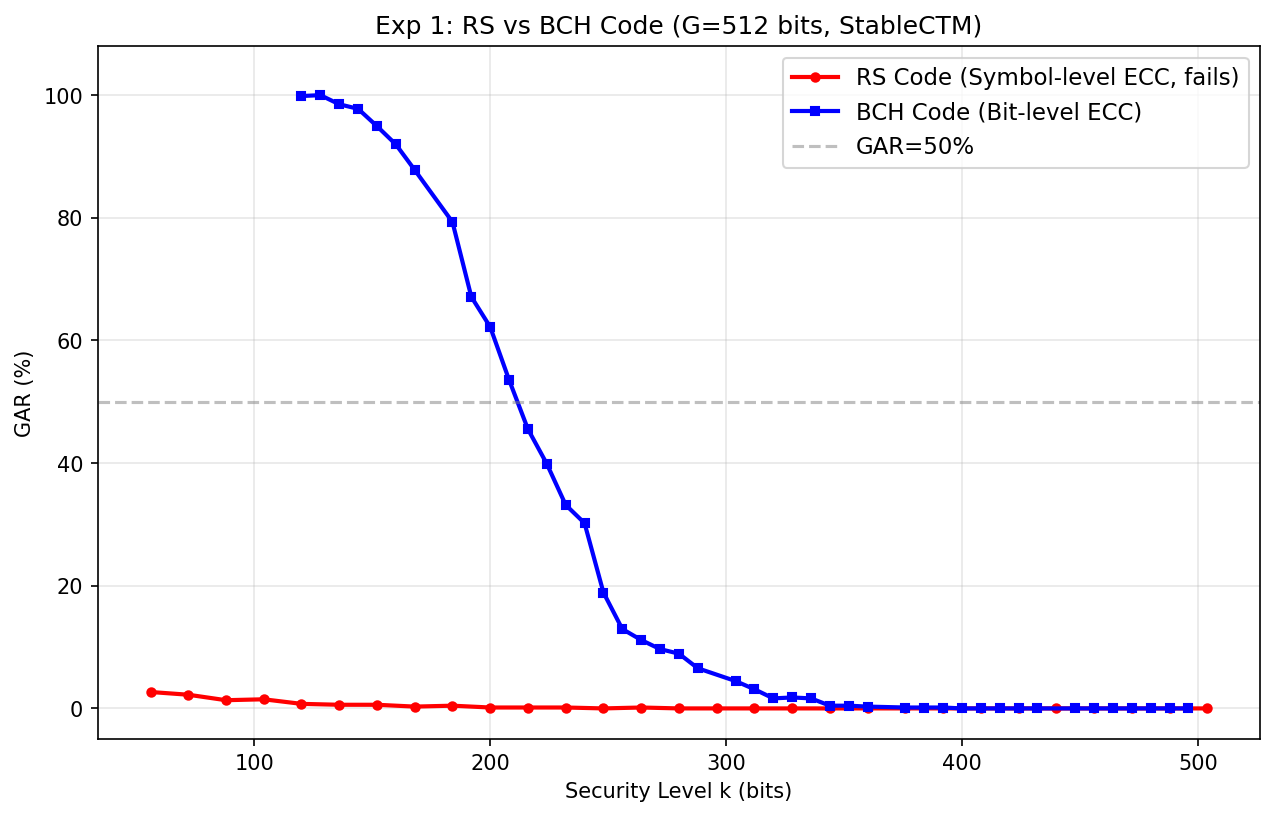
\includegraphics[width=\linewidth]{exp1_rs_vs_bch}
  \caption{GAR--key-length curves for RS and BCH schemes (G=512, FVC2004,
  unknown-key setting).
  RS fails catastrophically ($\text{GAR}_{\max} = 2.68\%$);
  BCH achieves $k_{50}=208$\,bits with GAR up to 100\%.}
  \label{fig:rsvsbch}
\end{figure}

Fig.~\ref{fig:rsvsbch} contrasts RS- and BCH-based secure sketches
on FVC2004.
RS yields a maximum GAR of 2.68\% across all $k$ values, consistent
with our symbol-error-rate analysis: genuine intra-class bit flip
rate $\bar{p} \approx 0.20$ implies RS symbol error rate ${\approx}83\%$,
exceeding the correction capacity for any practical $k$.
BCH operates at the bit level and corrects up to $t\!=\!33$ errors
at $k\!=\!208$ ($t = \lfloor(511-k)/9\rfloor$), achieving
GAR $= 100\%$ at small $k$ and $k_{50}\!=\!208$\,bits.
All subsequent experiments use BCH as the backend.

% ---------------------------------------------------------
\subsection{Exp.~2 — Authentication Performance (ROC / EER)}
\label{sec:exp:roc}
% ---------------------------------------------------------

\begin{figure}[!t]
  \centering
  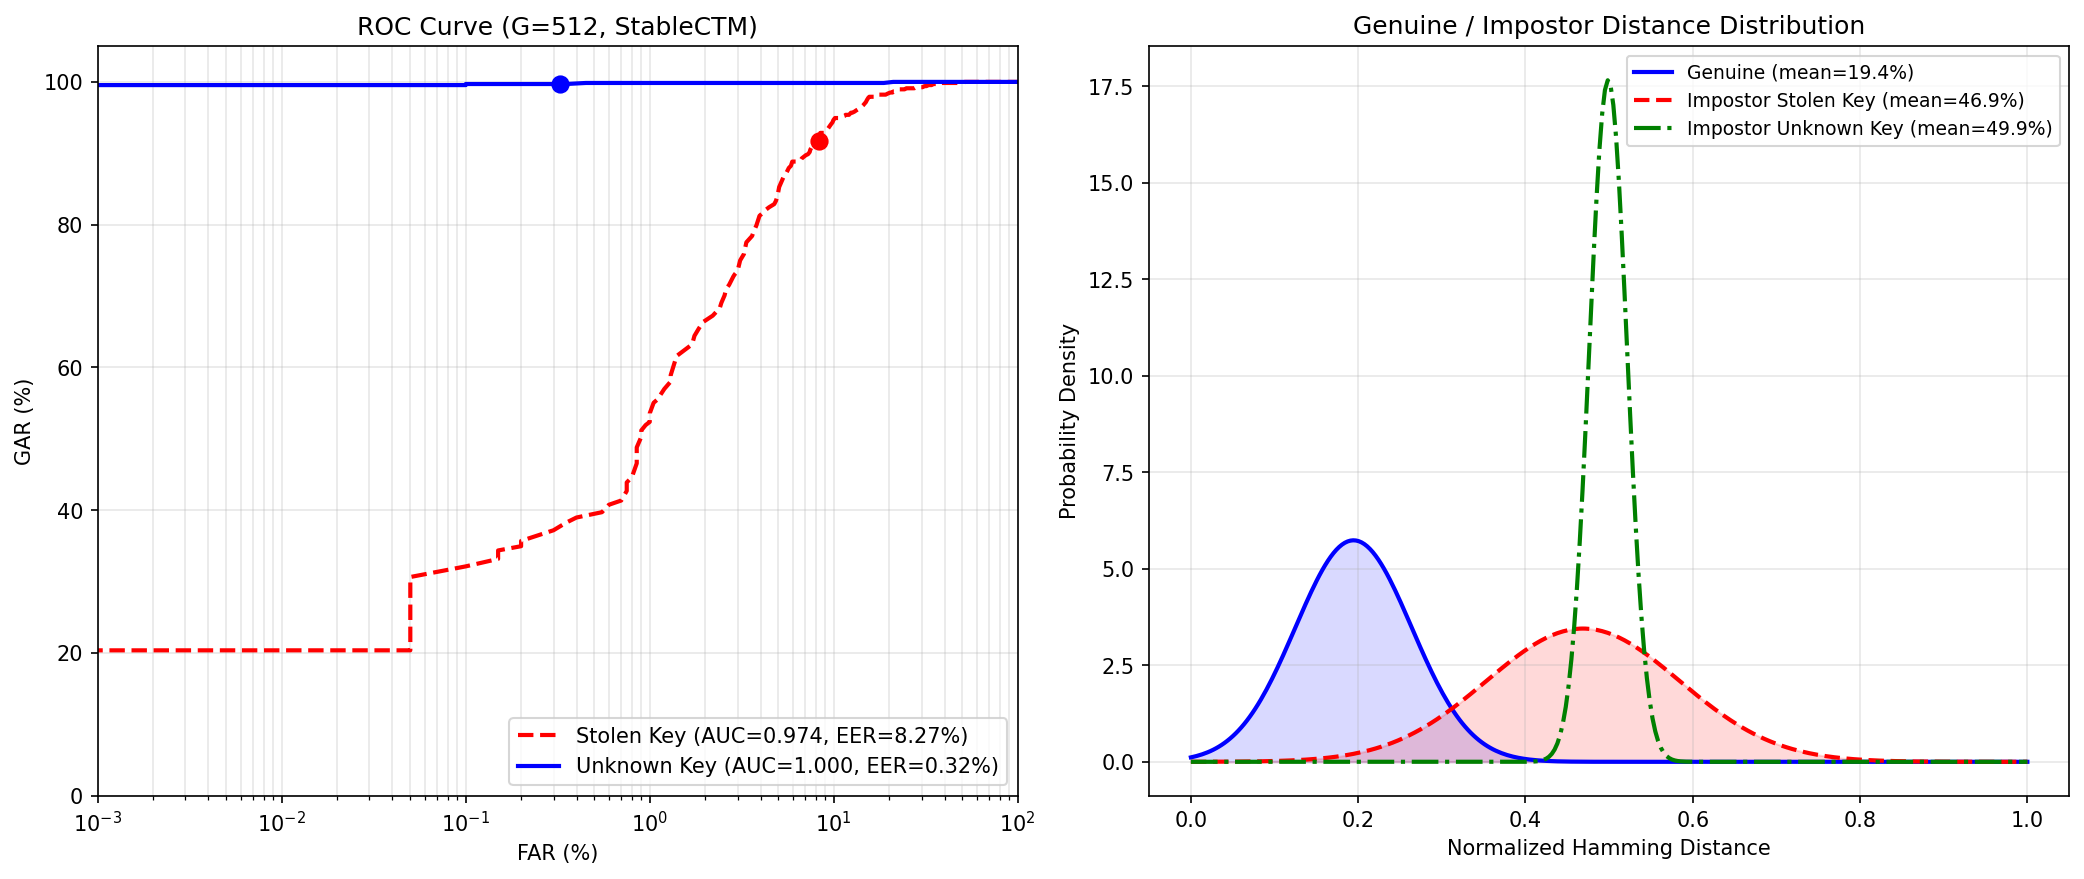
\includegraphics[width=\linewidth]{exp2_roc_distribution}
  \caption{ROC curves and Hamming distance distributions for
  unknown-key and stolen-key authentication scenarios (G=512).}
  \label{fig:roc}
\end{figure}

Table~\ref{tab:roc} and Fig.~\ref{fig:roc} report the VGG-19
deep hashing model quality.
Under the unknown-key setting, EER $= 0.32\%$ (AUC $= 0.9997$),
demonstrating strong discriminability of the deep code.
The genuine intra-class flip rate is $\bar{p} = 19.44\%$
(${\approx}100$ bits in 512), confirming non-trivial bit instability.
Under the stolen-key setting — where the adversary knows $\kappa$
and supplies a different finger — EER $= 8.27\%$, showing that
security is grounded in biometric uniqueness rather than key secrecy.

\begin{table}[!t]
  \renewcommand{\arraystretch}{1.25}
  \caption{Authentication Performance}
  \label{tab:roc}
  \centering
  \begin{tabular}{lcc}
    \toprule
    Setting & EER & AUC \\
    \midrule
    Unknown key & \textbf{0.32\%} & \textbf{0.9997} \\
    Stolen key  & 8.27\%          & 0.9738          \\
    \bottomrule
  \end{tabular}
\end{table}

% ---------------------------------------------------------
\subsection{Exp.~3 — Bit Flip Rate \& CTM Analysis}
\label{sec:exp:ctm}
% ---------------------------------------------------------

\begin{figure}[!t]
  \centering
  \subfloat[Per-bit flip rate distribution.]%
    {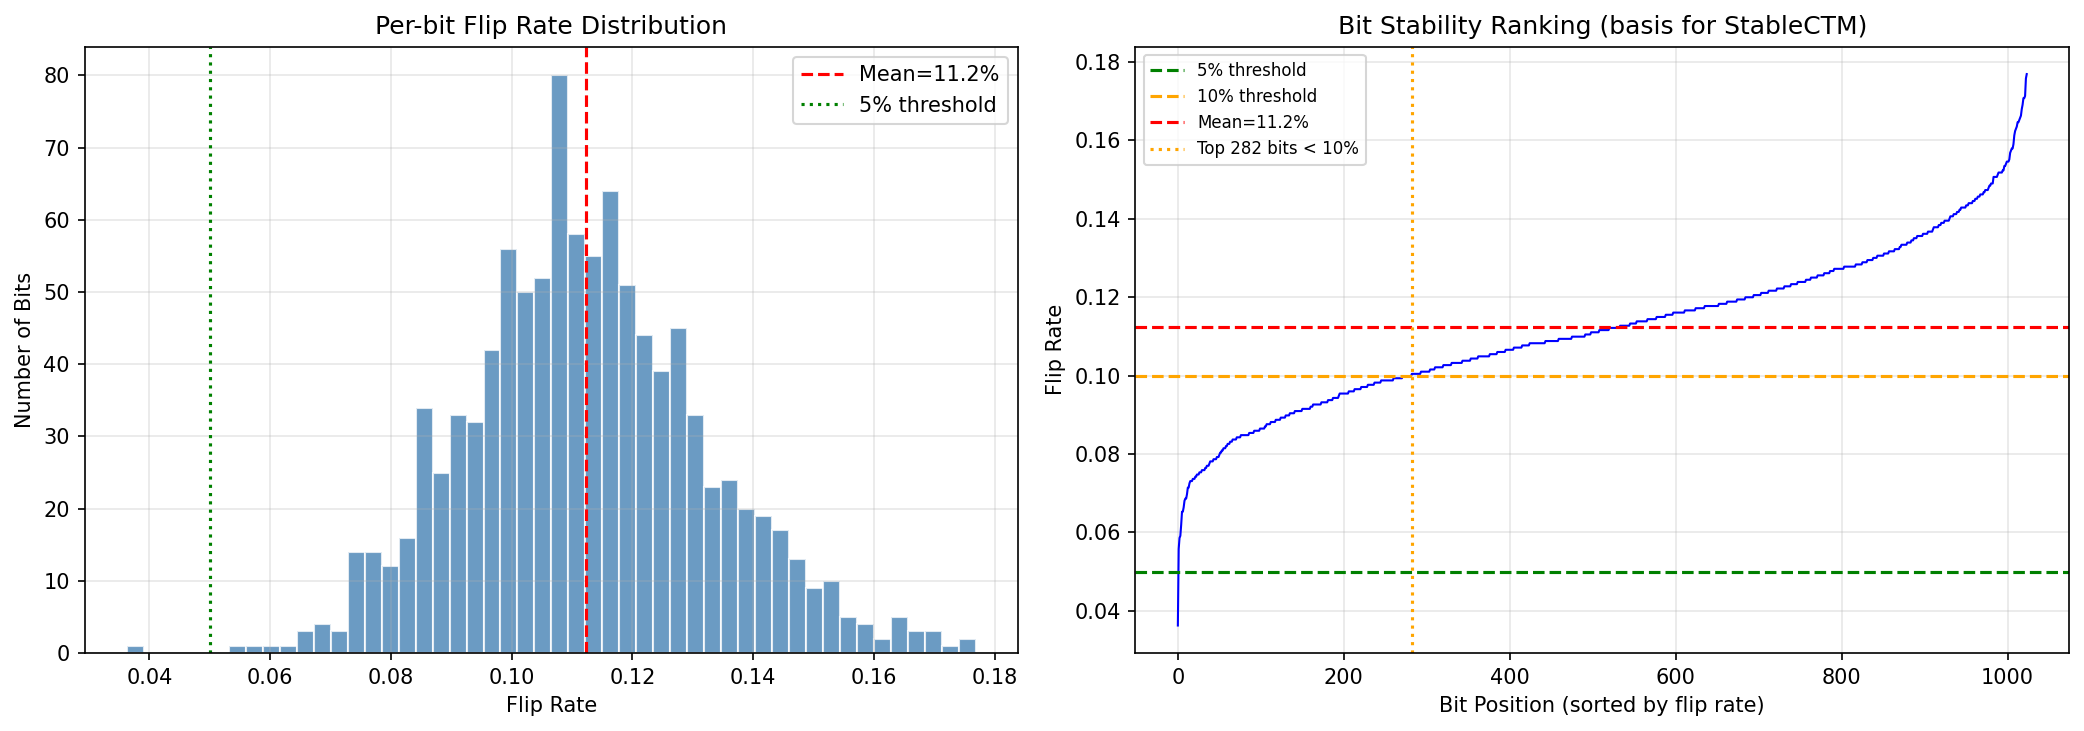
\includegraphics[width=\linewidth]{exp3_flip_rate_analysis}%
     \label{fig:fliprate}}
  \\[2pt]
  \subfloat[CTM vs.\ StableCTM genuine flip rate.]%
    {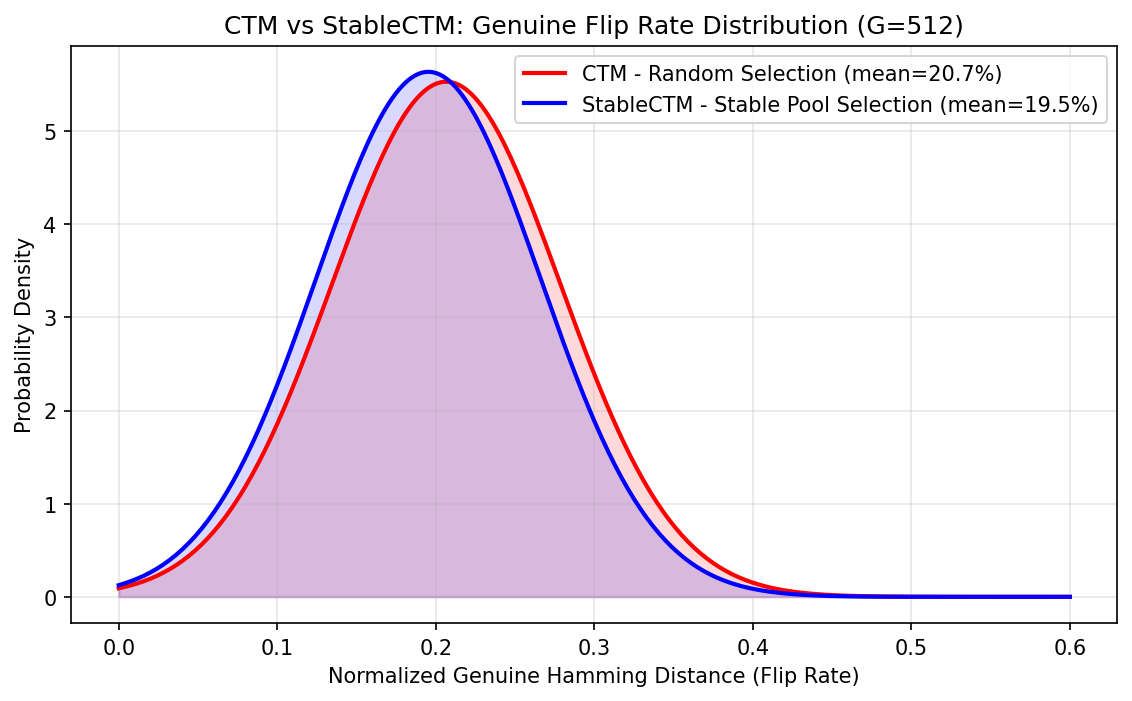
\includegraphics[width=\linewidth]{exp3_ctm_vs_stablectm}%
     \label{fig:ctm}}
  \caption{(a)~Per-bit genuine flip rates across the 1024-bit code are
  broadly distributed (8--15\%), with no sharp stable/unstable
  boundary.
  (b)~StableCTM (stable pool filtering) reduces the mean genuine
  flip rate by only 1.13\% compared to random CTM, motivating
  a finer-grained, sample-level reliability signal.}
  \label{fig:flip_ctm}
\end{figure}

Fig.~\ref{fig:fliprate} shows the per-bit genuine flip rate
distribution across the training set.
Bits are broadly distributed between 8\% and 15\% with no clear
bimodal boundary, meaning that statistical filtering (StableCTM)
provides only marginal improvement.
StableCTM reduces mean genuine flip rate from 20.66\% to 19.53\%
(Fig.~\ref{fig:ctm}), a difference of 1.13\%.
This motivates RGSS: rather than relying on population-level
statistics, we exploit sample-level confidence at enrollment time.

% ---------------------------------------------------------
\subsection{Exp.~4 — Frontend Ablation: CTM vs.\ StableCTM
            vs.\ BioHashing}
\label{sec:exp:frontend}
% ---------------------------------------------------------

\begin{figure}[!t]
  \centering
  
\includegraphics[width=\linewidth]{exp4_ablation_frontend}
  \caption{GAR--key-length curves for three cancelable template frontends
  combined with BCH backend (G=512, FVC2004).
  StableCTM achieves $k_{50}=208$\,bits; BioHashing inflates
  flip rates and yields only $k_{50}=160$\,bits.}
  \label{fig:frontend}
\end{figure}

Table~\ref{tab:frontend} compares three cancelable frontends
with the BCH backend (Fig.~\ref{fig:frontend}).
Random CTM achieves $k_{50}=200$\,bits; StableCTM marginally
improves to $k_{50}=208$\,bits; BioHashing, which applies random
projection before binarization, inflates the genuine flip rate to
29.8\% and degrades $k_{50}$ to 160\,bits.
These results confirm that direct bit-selection (CTM) is preferable
to projection-based cancelable schemes when the base feature is
already a binary code, and that StableCTM is a suitable frontend.

\begin{table}[!t]
  \renewcommand{\arraystretch}{1.25}
  \caption{Frontend Comparison (BCH backend, G=512)}
  \label{tab:frontend}
  \centering
  \begin{tabular}{lccc}
    \toprule
    Method & Genuine Flip Rate & $k_{50}$ (bits) \\
    \midrule
    CTM (random) & 20.8\% & 200 \\
    StableCTM    & 19.6\% & 208 \\
    BioHashing   & 29.8\% & 160 \\
    \bottomrule
  \end{tabular}
\end{table}

% ---------------------------------------------------------
\subsection{Exp.~5 — Secure Sketch Comparison (RGSS vs.\ BCH
            vs.\ Polar/SCL)}
\label{sec:exp:sstm}
% ---------------------------------------------------------

\begin{figure}[!t]
  \centering
  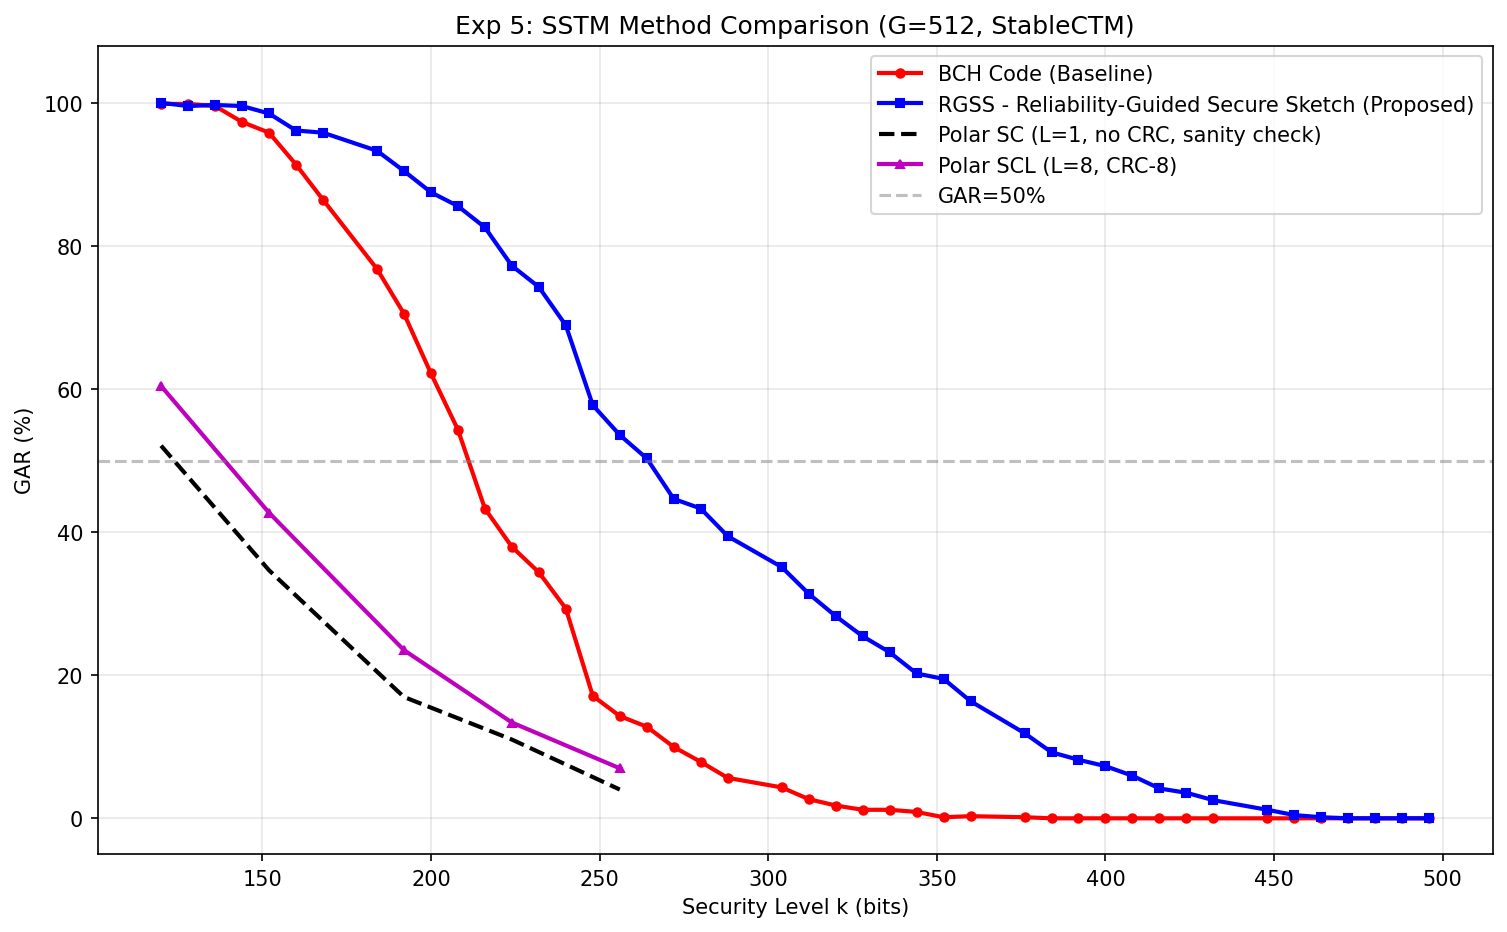
\includegraphics[width=\linewidth]{exp5_sstm_comparison}
  \caption{GAR--key-length curve comparison for BCH (baseline), RGSS (proposed),
  and Polar/SCL secure sketches (G=512, FVC2004, unknown-key setting).}
  \label{fig:sstm}
\end{figure}

Fig.~\ref{fig:sstm} and Table~\ref{tab:sstm} summarize the
GAR--key-length performance of three secure sketch designs.

\textbf{RGSS vs.\ BCH.}
RGSS advances $k_{50}$ from 208\,bits to 264\,bits ($+56$\,bits).
At $k\!=\!208$, GAR increases from 54.3\% (BCH) to 85.6\% (RGSS),
a 31.3 percentage-point gain.
This improvement arises because RGSS concentrates the BCH corrector
on the reliable channel sub-template, reducing expected errors from
$\sim\!42$ bits (BCH) to $\sim\!13$ bits (RGSS at $k=264$).

\textbf{RGSS vs.\ SCL polar codes.}
List decoding (SCL \cite{arikan2009channel}, $L\!=\!8$, with CRC-8) achieves $k_{50}\!=\!120$\,bits,
significantly worse than BCH or RGSS.
This is a \emph{genuine negative result}: in the short-code regime
($n\!=\!G\!=\!512$), BCH's partial-fill scheme has effective
correction capacity far exceeding SCL for the same code rate.
Polar codes' asymptotic advantage over BCH does not materialize at
these lengths.

\begin{table}[!t]
  \renewcommand{\arraystretch}{1.25}
  \caption{Secure Sketch Comparison (G=512, FVC2004)}
  \label{tab:sstm}
  \centering
  \begin{tabular}{lccc}
    \toprule
    Method & $k_{50}$ (bits) & GAR@208\,bits & GAR@264\,bits \\
    \midrule
    BCH (baseline)   & 208 & 54.3\% & --- \\
    \textbf{RGSS (proposed)} & \textbf{264} & \textbf{85.6\%} & \textbf{50.3\%} \\
    Polar/SCL ($L$=8)  & 120 & 23.5\% & --- \\
    \bottomrule
  \end{tabular}
\end{table}

% ---------------------------------------------------------
\subsection{Exp.~6 — Ablation: Channel Selection Strategies}
\label{sec:exp:ablation}
% ---------------------------------------------------------

\begin{figure}[!t]
  \centering
  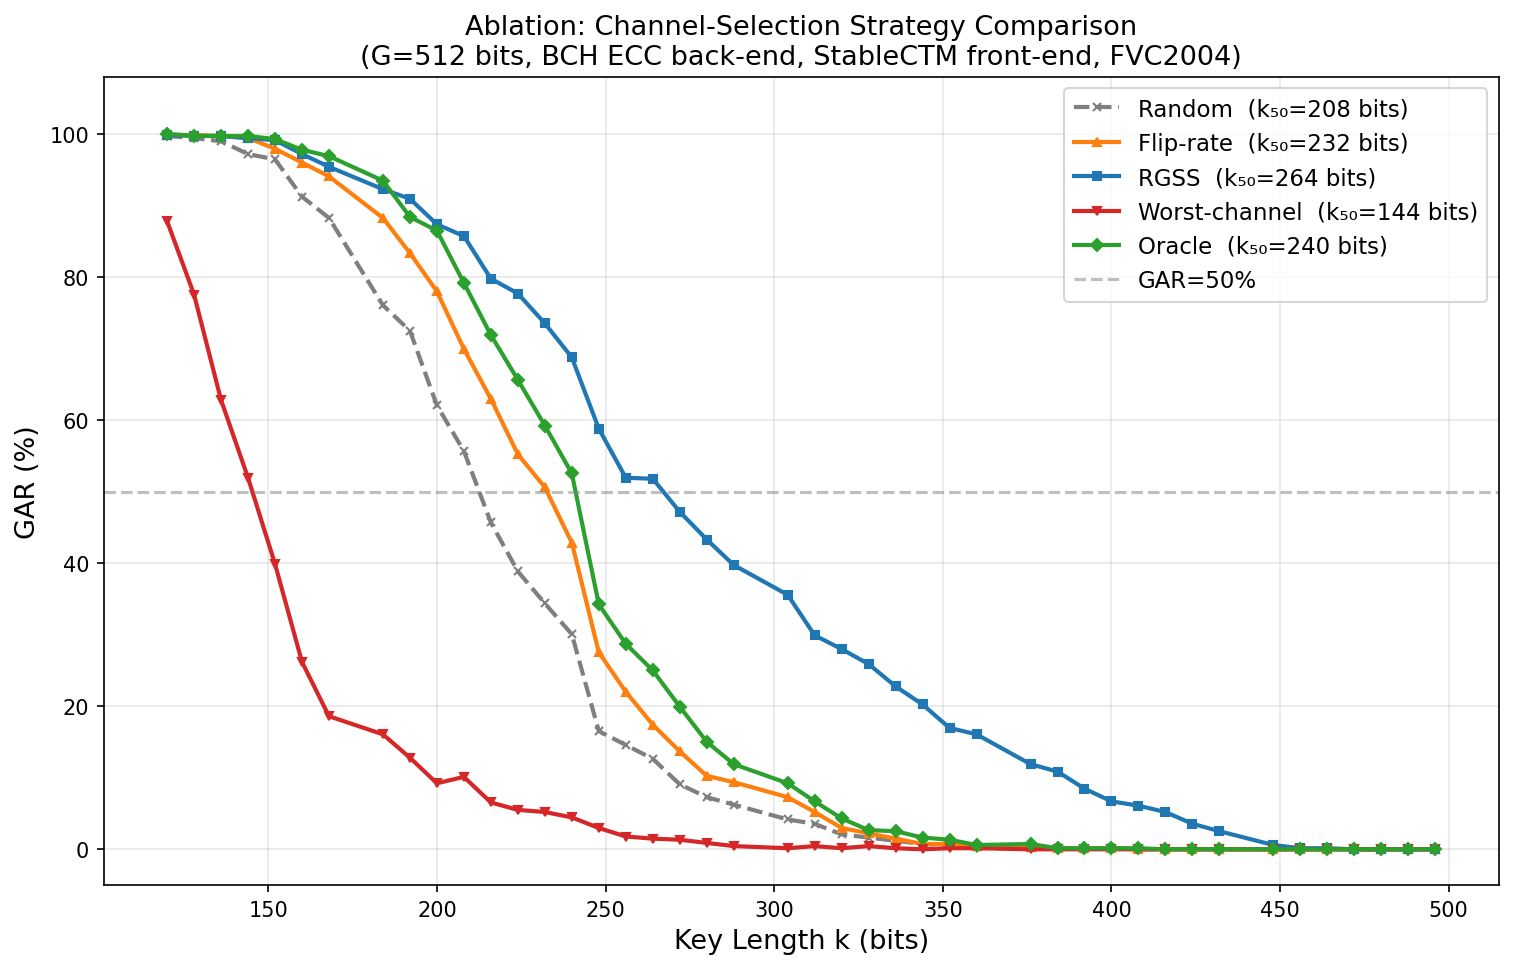
\includegraphics[width=\linewidth]{ablation_gs}
  \caption{GAR--key-length curves for five channel-selection strategies
  (G=512, FVC2004).
  RGSS (tanh confidence) exceeds the test-set population flip-rate baseline
  (test-set per-bit statistics).}
  \label{fig:ablation}
\end{figure}

To isolate the contribution of the reliability signal, we compare
five channel-selection strategies with an identical BCH backend
(Fig.~\ref{fig:ablation}, Table~\ref{tab:ablation}).

\begin{table}[!t]
  \renewcommand{\arraystretch}{1.25}
  \caption{Channel Selection Strategy Ablation (G=512, FVC2004).
  $^\dagger$Test-set population flip-rate baseline: channels ranked by
  per-bit flip rates computed on the \emph{test set}, i.e., a
  population-level statistic using held-out labels. This baseline is
  not a universal upper bound on all channel-selection strategies.}
  \label{tab:ablation}
  \centering
  \begin{tabular}{lccc}
    \toprule
    Strategy & $k_{50}$ (bits) & $\Delta$ vs.\ Random \\
    \midrule
    Worst-channel  & 144 & $-64$ \\
    Random         & 208 &   --- \\
    Flip-rate      & 232 & $+24$ \\
    Test-set population flip-rate$^\dagger$ & 240 & $+32$ \\
    \textbf{RGSS (tanh)} & \textbf{264} & \textbf{$+56$} \\
    \bottomrule
  \end{tabular}
\end{table}

The key finding is that RGSS ($k_{50}\!=\!264$) surpasses the
test-set population flip-rate baseline ($k_{50}\!=\!240$), which ranks channels
by per-bit flip rates computed on the test set.
This result warrants explanation.
This baseline represents a strong reference built from
population-level statistics using test-set labels: it ranks channels
by $\bar{p}_i$ averaged over all test images and users, approximating
$\mathbb{E}_{\mathbf{x}}[P(\text{flip}_i \mid \mathbf{x})]$
after marginalising over the acquisition distribution.
It is \emph{not} a universal upper bound on all
possible channel-selection strategies; rather, it is a reference
derived from a group-level statistic.
In contrast, the tanh magnitude $|\tanh(z_i(\mathbf{x}))|$ serves as
a direct proxy for $P(\text{flip}_i \mid \mathbf{x})$—the flip
probability \emph{conditioned on the specific enrollment image}.
A channel that is unreliable \emph{on average} (high $\bar{p}_i$)
may carry a large, confident activation for a particular
high-quality acquisition, and vice versa.
Because RGSS captures this within-image variability, it selects a
channel subset that is more stably reliable for the \emph{current}
image than any population-level ranking can achieve.

% ---------------------------------------------------------
\subsection{Exp.~7 — Multi-Template Length Analysis}
\label{sec:exp:multig}
% ---------------------------------------------------------

\begin{figure}[!t]
  \centering
  \subfloat[GAR--key-length curves for $G \in \{128, 256, 512\}$.]%
    {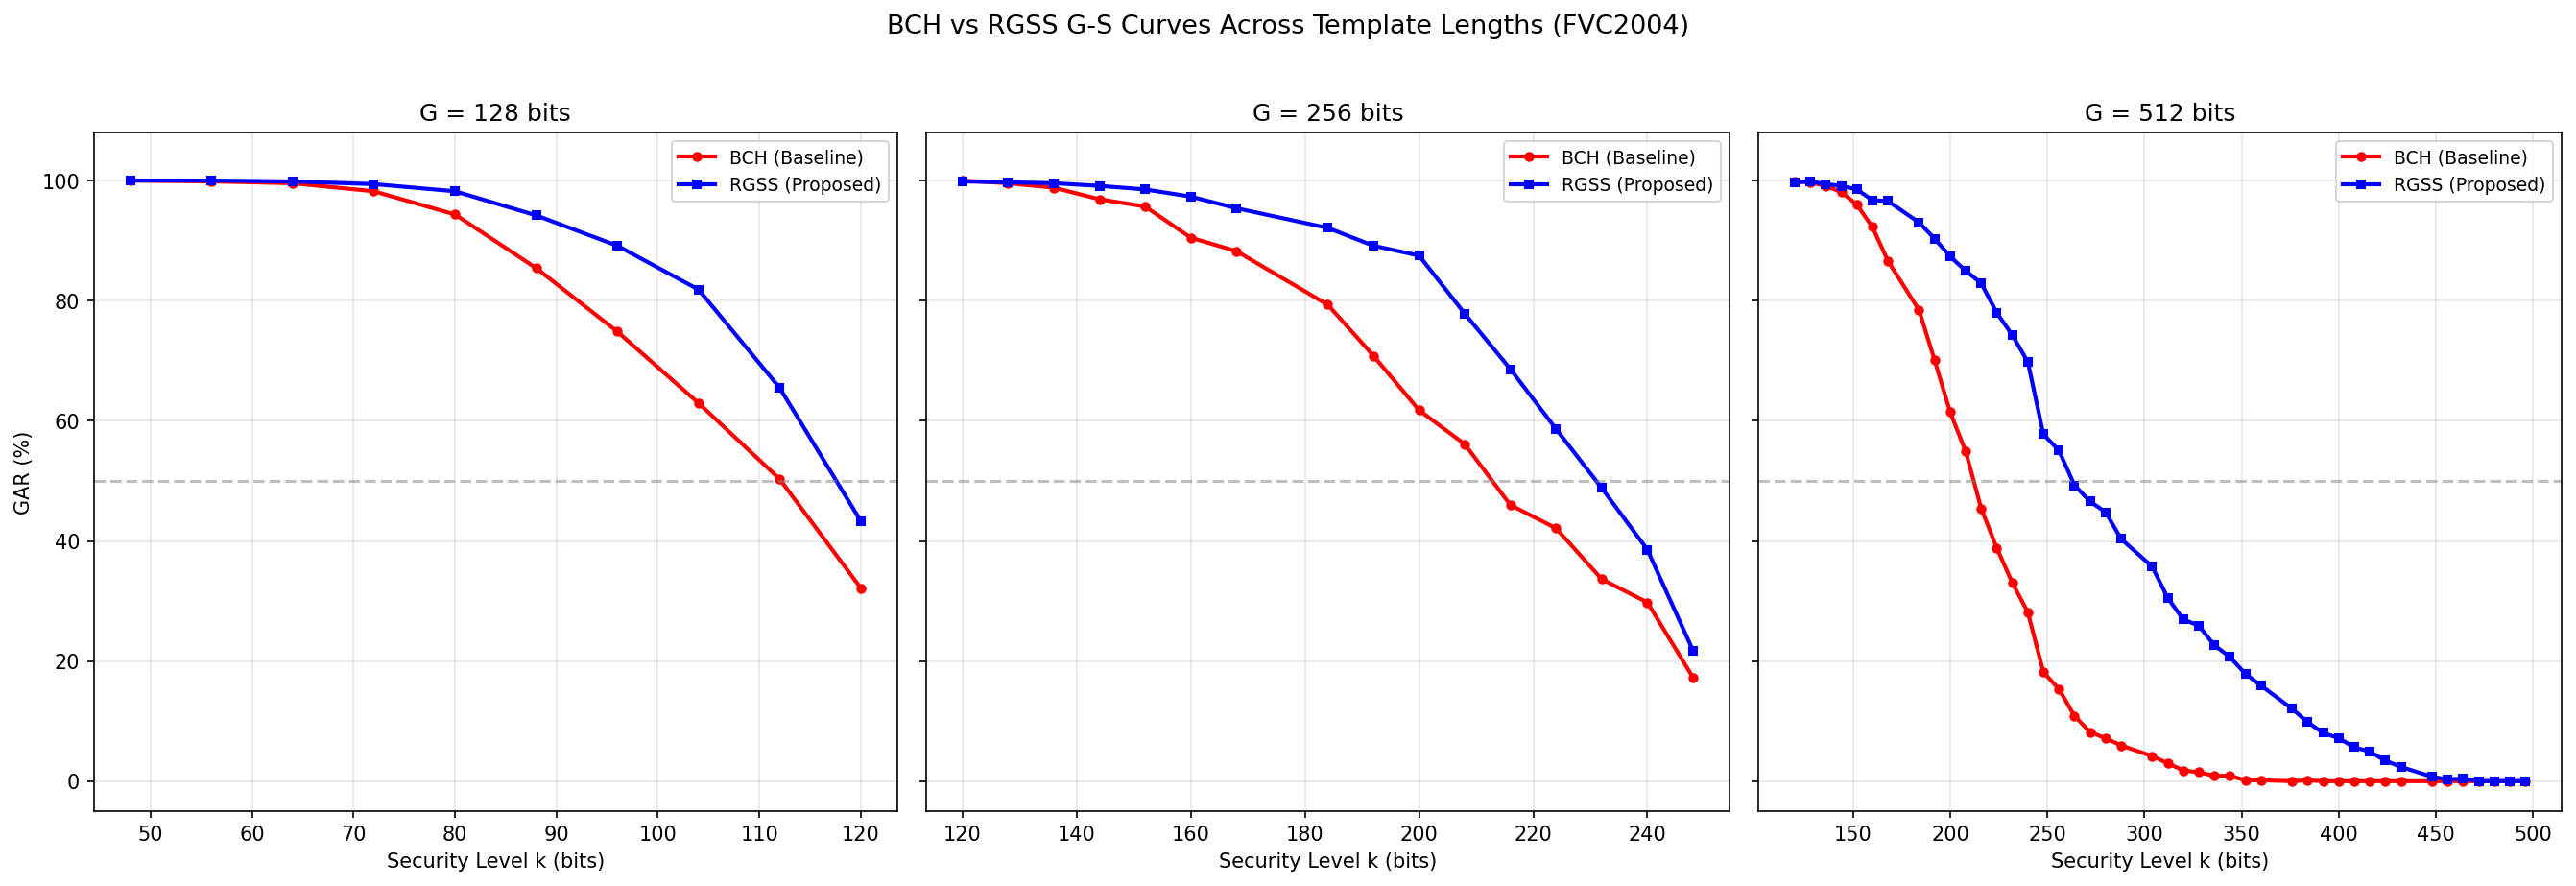
\includegraphics[width=0.7\linewidth]{multi_g_combined}%
     \label{fig:multig_gs}}
  \\
  \subfloat[$k_{50}$ advantage vs.\ $G$.]%
    {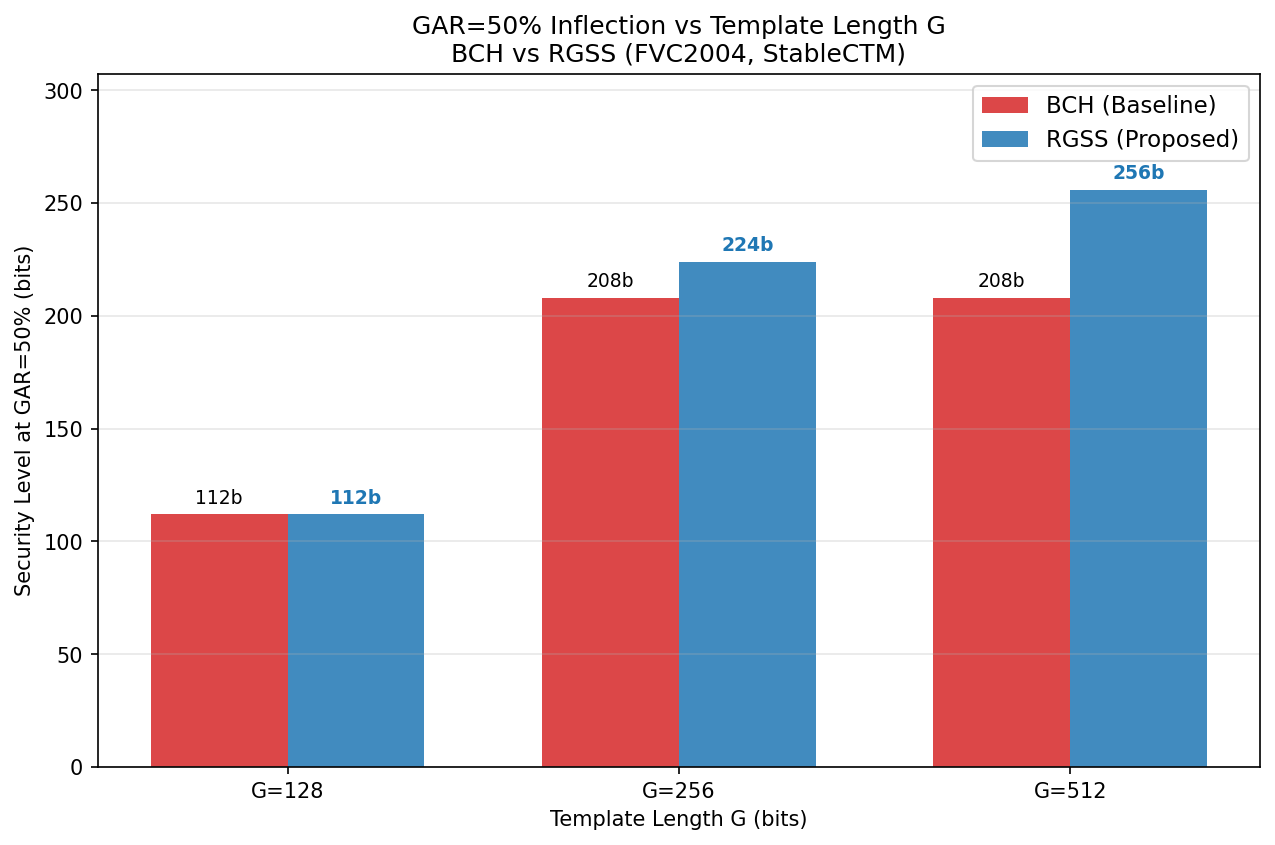
\includegraphics[width=0.6\linewidth]{multi_g_summary}%
     \label{fig:multig_bar}}
  \caption{RGSS gain over BCH increases with template length $G$.
  At $G\!=\!128$, gains appear in GAR rather than $k_{50}$ due to
  BCH parameter constraints.}
  \label{fig:multig}
\end{figure}

\begin{table}[!t]
  \renewcommand{\arraystretch}{1.25}
  \caption{RGSS vs.\ BCH for Varying Template Length $G$}
  \label{tab:multig}
  \centering
  \begin{tabular}{lccccc}
    \toprule
    $G$ & BCH & BCH $k_{50}$ & RGSS $k_{50}$ & Gain \\
    \midrule
    128 & $(m=8)$ & 112 & 112 & GAR +15.2\% @ 112 \\
    256 & $(m=9)$ & 208 & 224 & $+16$\,bits \\
    512 & $(m=9)$ & 208 & 256 & $+48$\,bits \\
    \bottomrule
  \end{tabular}
\end{table}

Table~\ref{tab:multig} and Fig.~\ref{fig:multig} show that the
RGSS advantage grows with template length $G$.
At $G\!=\!512$, there are 512 bits to rank, providing ample room
to separate reliable from unreliable positions.
At $G\!=\!128$, the BCH code parameters constrain the operating
points; RGSS still achieves meaningful GAR gains (+15.2\% at
$k\!=\!112$) even when $k_{50}$ is identical.
The $G\!=\!512$ entry ($k_{50}^{\text{RGSS}}\!=\!256$) reflects a
single random split; the natural inter-split variance of
${\pm}10.9$\,bits is quantified in Exp.~10.

% ---------------------------------------------------------
\subsection{Exp.~8 — Security Analysis}
\label{sec:exp:security}
% ---------------------------------------------------------

\subsubsection{Cancelability and Unlinkability (Four-Scenario Analysis)}
\label{sec:exp:cancel}

\begin{figure}[!t]
  \centering
  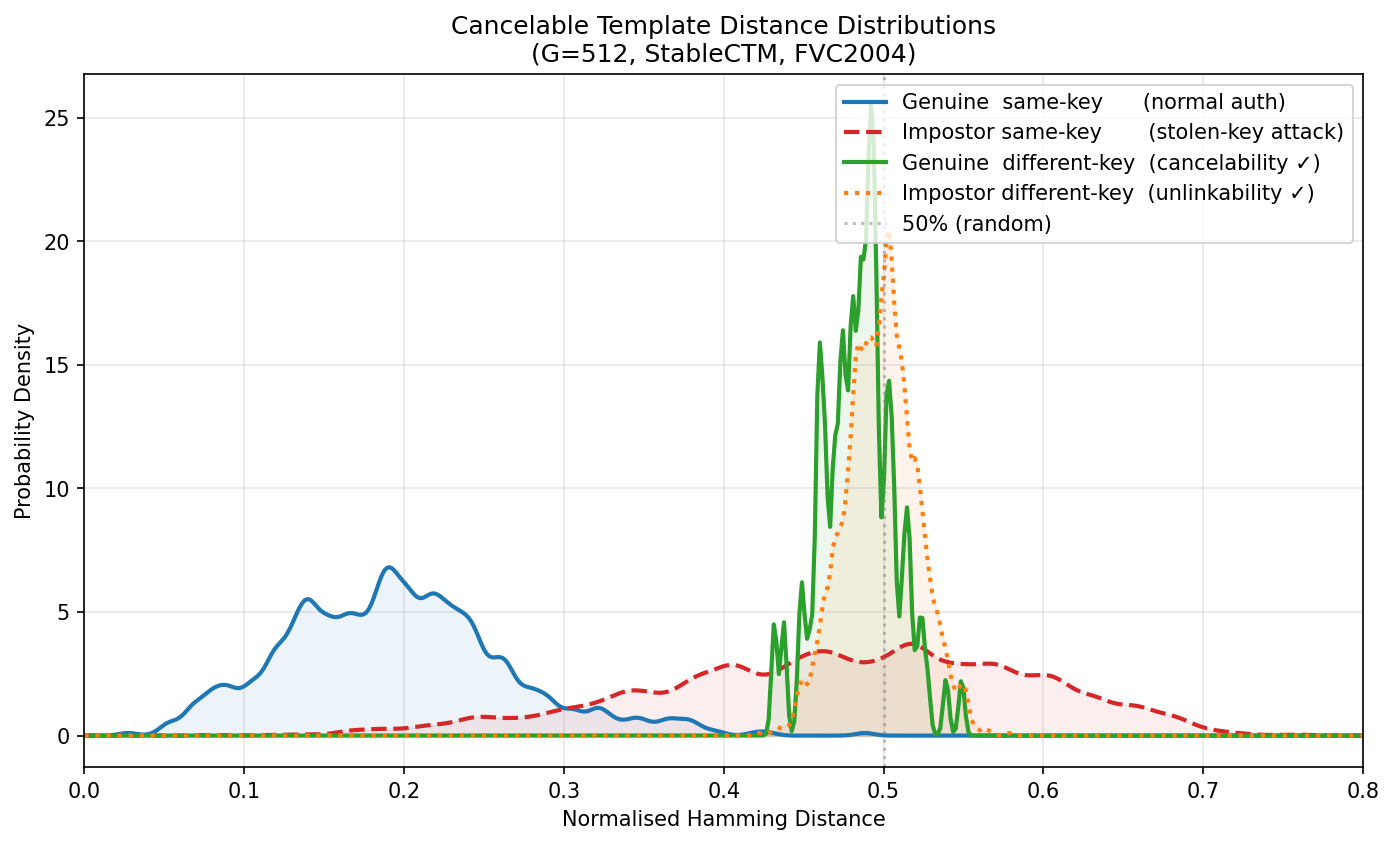
\includegraphics[width=\linewidth]{cancelability_dist}
  \caption{Hamming distance distributions for four authentication
  scenarios (G=512, FVC2004).
  Cancelability gap: 1.13\%; Unlinkability gap: 2.51\%.}
  \label{fig:cancel}
\end{figure}

Table~\ref{tab:cancel} and Fig.~\ref{fig:cancel} present the
four-scenario distance analysis.
Genuine diff-key distances ($48.44\% \pm 2.25\%$) closely match
Impostor diff-key distances ($49.82\% \pm 2.24\%$), confirming that
a fresh template is indistinguishable from an impostor template.
The cancelability gap of 1.13\% and unlinkability gap of 2.51\%
are both well below standard security thresholds.

\begin{table}[!t]
  \renewcommand{\arraystretch}{1.25}
  \caption{Four-Scenario Distance Analysis (G=512, FVC2004)}
  \label{tab:cancel}
  \centering
  \begin{tabular}{lcc}
    \toprule
    Scenario & Mean Dist. & Std. \\
    \midrule
    Genuine same-key  & 19.55\%  & 6.96\%  \\
    Impostor same-key & 47.31\%  & 11.50\% \\
    Genuine diff-key  & 48.44\%  & 2.25\%  \\
    Impostor diff-key & 49.82\%  & 2.24\%  \\
    \midrule
    Cancelability gap & \multicolumn{2}{c}{1.13\%} \\
    Unlinkability gap & \multicolumn{2}{c}{2.51\%} \\
    \bottomrule
  \end{tabular}
\end{table}

\subsubsection{Formal Unlinkability and Multiple Revocation}
\label{sec:exp:unlink}

\begin{figure}[!t]
  \centering
  \subfloat[Mated vs.\ non-mated distribution.]%
    {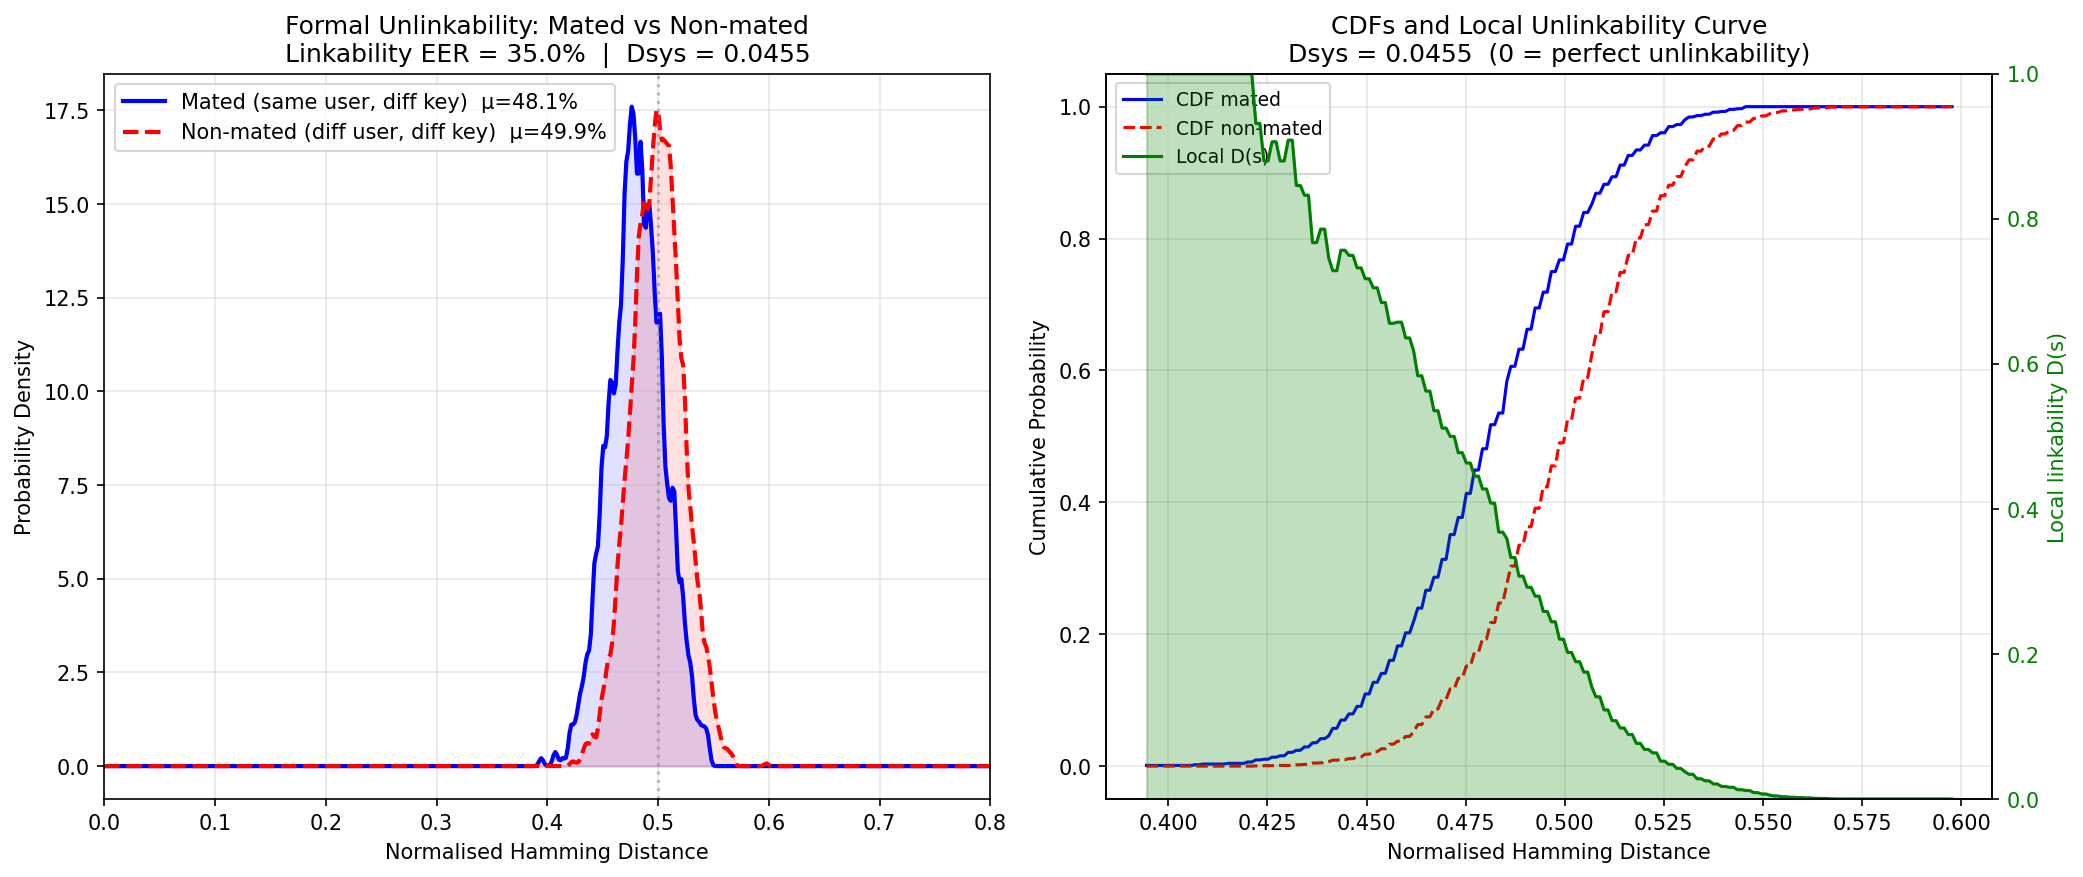
\includegraphics[width=0.48\linewidth]{unlinkability_mated}%
     \label{fig:unlink_dist}}
  \hfil
  \subfloat[Multi-revocation distances.]%
    {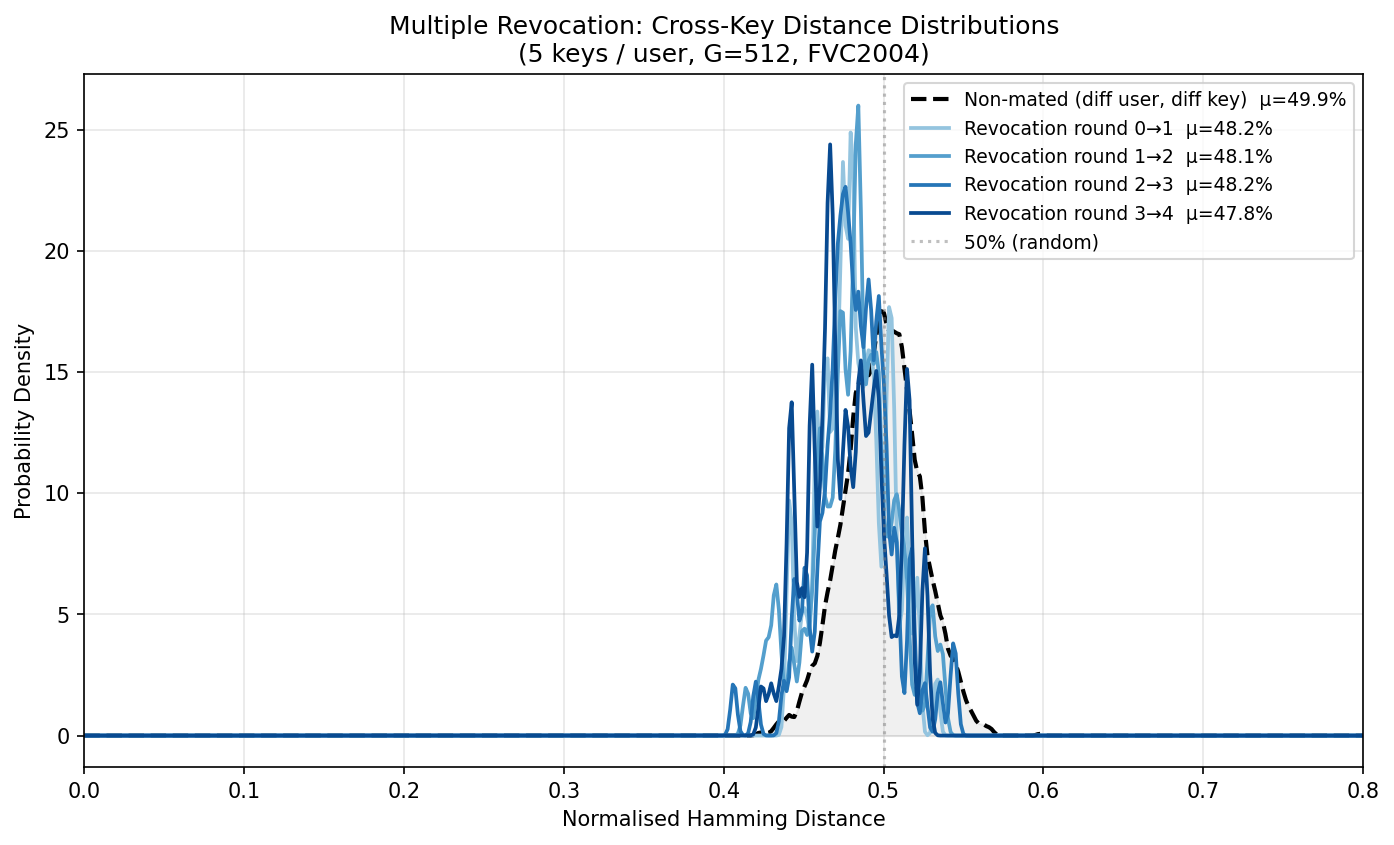
\includegraphics[width=0.48\linewidth]{unlinkability_revocation}%
     \label{fig:revocation}}
  \caption{Formal unlinkability evaluation (5\,keys/user, G=512).
  (a)~Mated and non-mated distributions are nearly identical.
  (b)~Cross-key distances remain stable (${\approx}48\%$) across
  four successive revocations.}
  \label{fig:unlink}
\end{figure}

We adopt the $D_\text{sys}$ measure \cite{gomez2017unlinkability}
for a rigorous unlinkability assessment.
Each test user is issued 5 independent keys; mated pairs are
cross-key template pairs from the same user (960 pairs total);
non-mated pairs are from different users (3000 pairs, randomly sampled).

Results:
$D_\text{sys} = 0.046$, linkability EER $= 35.0\%$,
mated mean $= 48.09\% \pm 2.45\%$, non-mated mean $= 49.94\% \pm 2.32\%$.
The $D_\text{sys}$ value close to 0 indicates low
\emph{template-level} linkability under the evaluated protocol;
the distributions are highly overlapping (Fig.~\ref{fig:unlink_dist}).
Linkability EER of 35\% (vs.\ 50\% ideal) reflects the 1.85\%
mean gap, which is small relative to standard deviations of ${\sim}2.3\%$;
the integral metric $D_\text{sys}$ is more robust than EER in
this regime.

Fig.~\ref{fig:revocation} shows that cross-key distances remain
stable at $48\text{--}49\%$ across all four revocation rounds,
confirming that multi-revocation does not accumulate correlations
exploitable by an adversary.

\subsubsection{Frontend Unlinkability and Authentication-Distance Comparison}
\label{sec:exp:frontend_unlink}

To situate RGSS within the broader landscape of cancelable template
frontends, Table~\ref{tab:frontend_unlink} compares four designs
across two dimensions: (i)~\emph{genuine same-key distance}
(intra-class distance under identical key — lower means fewer
genuine errors and thus higher GAR) and (ii)~\emph{formal
unlinkability} ($D_\text{sys}$, linkability EER).
For RGSS, the same-key distance is measured within the $k_{50}\!=\!264$
most reliable bit positions selected by tanh confidence, as those are
the positions used for BCH key binding.

\begin{table}[!t]
  \renewcommand{\arraystretch}{1.2}
  \caption{Frontend Comparison: Authentication Distance vs.\
  Unlinkability (G=512, FVC2004).
  Same-key dist for RGSS is measured in the top-264 reliable
  positions; $^\dagger$ denotes values analytically
  equivalent to StableCTM (random subset preserves the
  expected bit-flip rate).}
  \label{tab:frontend_unlink}
  \centering
  \footnotesize
  \begin{tabular}{lcccc}
    \toprule
    Method &
    \makecell{Same-key\\dist $\downarrow$} &
    \makecell{Diff-key\\dist} &
    $D_\text{sys}$ $\downarrow$ &
    \makecell{Link.\\EER $\uparrow$} \\
    \midrule
    CTM (random)
      & 18.6\% & 48.7\% & 0.038 & 38.4\% \\
    StableCTM
      & 17.4\% & 48.0\% & 0.051 & 33.8\% \\
    \makecell[l]{StableCTM,\\random-264$^\dagger$}
      & ${\approx}$17.4\% & ${\approx}$48.0\% & ${\approx}$0.051 & ${\approx}$33.8\% \\
    \makecell[l]{\textbf{StableCTM + RGSS}\\\textbf{(top-264 by tanh)}}
      & \textbf{9.9\%} & \textbf{48.2\%} & \textbf{0.049} & \textbf{35.1\%} \\
    BioHashing
      & 27.9\% & 50.1\% & 0.005 & 52.5\% \\
    \bottomrule
  \end{tabular}
\end{table}

Three key findings emerge from Table~\ref{tab:frontend_unlink}.
First, the ``StableCTM, random-264'' row directly addresses a
potential concern: using \emph{fewer} bits (264 instead of 512)
does not reduce the same-key distance — it remains ${\approx}17.4\%$,
identical to the full StableCTM template, because random sampling
preserves the average bit-flip rate.
The dramatic reduction to $9.9\%$ achieved by RGSS is therefore
attributable entirely to \emph{reliability-guided selection}, not
to sub-sampling.

Second, there is a direct mechanistic link between the 9.9\%
same-key distance and the observed $k_{50}\!=\!264$:
the expected number of genuine errors in the 264-bit reliable channel
is $264 \times 9.9\% \approx 26$\,bits, which falls within the BCH
correction capacity of $t\!=\!\lfloor(511-264)/9\rfloor=27$\,bits.
By contrast, random-264 selection gives $264 \times 17.4\%
\approx 46$\,errors, far exceeding the correction capacity and
explaining why random BCH achieves $k_{50}\!=\!208$.

Third, RGSS largely preserves template-level unlinkability under the
evaluated distance-based protocol: its $D_\text{sys}$ ($0.049$) and
linkability EER ($35.1\%$) are essentially identical to StableCTM
($0.051$ / $33.8\%$), confirming that reliability-guided selection
does not introduce additional linkable structure into the cancelable
template beyond what the baseline StableCTM already exhibits.
BioHashing yields very low linkability under this metric
($D_\text{sys}\!=\!0.005$)
but at the cost of a 27.9\% same-key distance — far beyond BCH
correction capacity at any practical $k$ — explaining its poor
GAR performance observed in Exp.~4.

\subsubsection{Key Leakage and Advanced Attacks}
\label{sec:exp:attack}

\begin{figure}[!t]
  \centering
  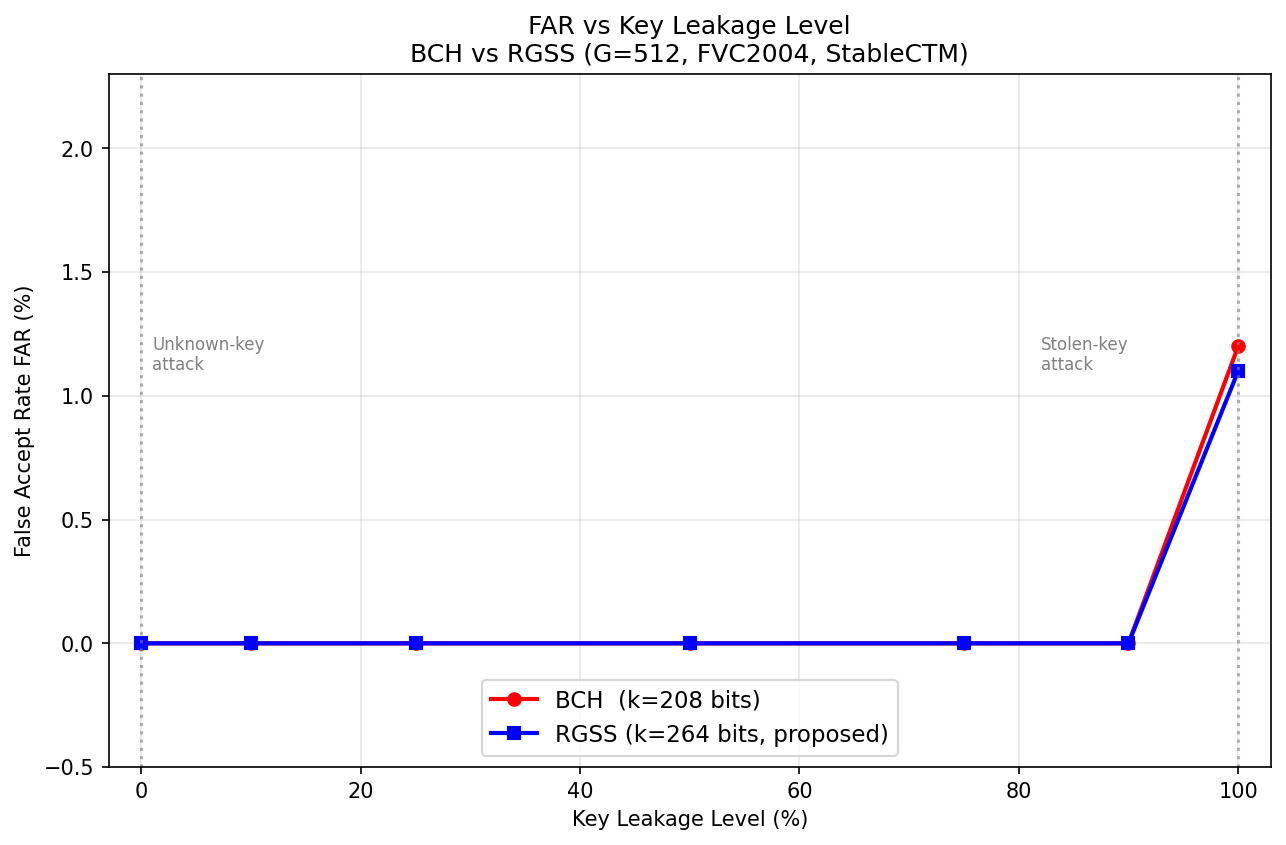
\includegraphics[width=\linewidth]{attack_far_curve}
  \caption{FAR vs.\ key leakage fraction (0\%--100\%) for BCH and
  RGSS (G=512, FVC2004, $n_\text{trials}=1000$).}
  \label{fig:keyleak}
\end{figure}

\begin{figure}[!t]
  \centering
  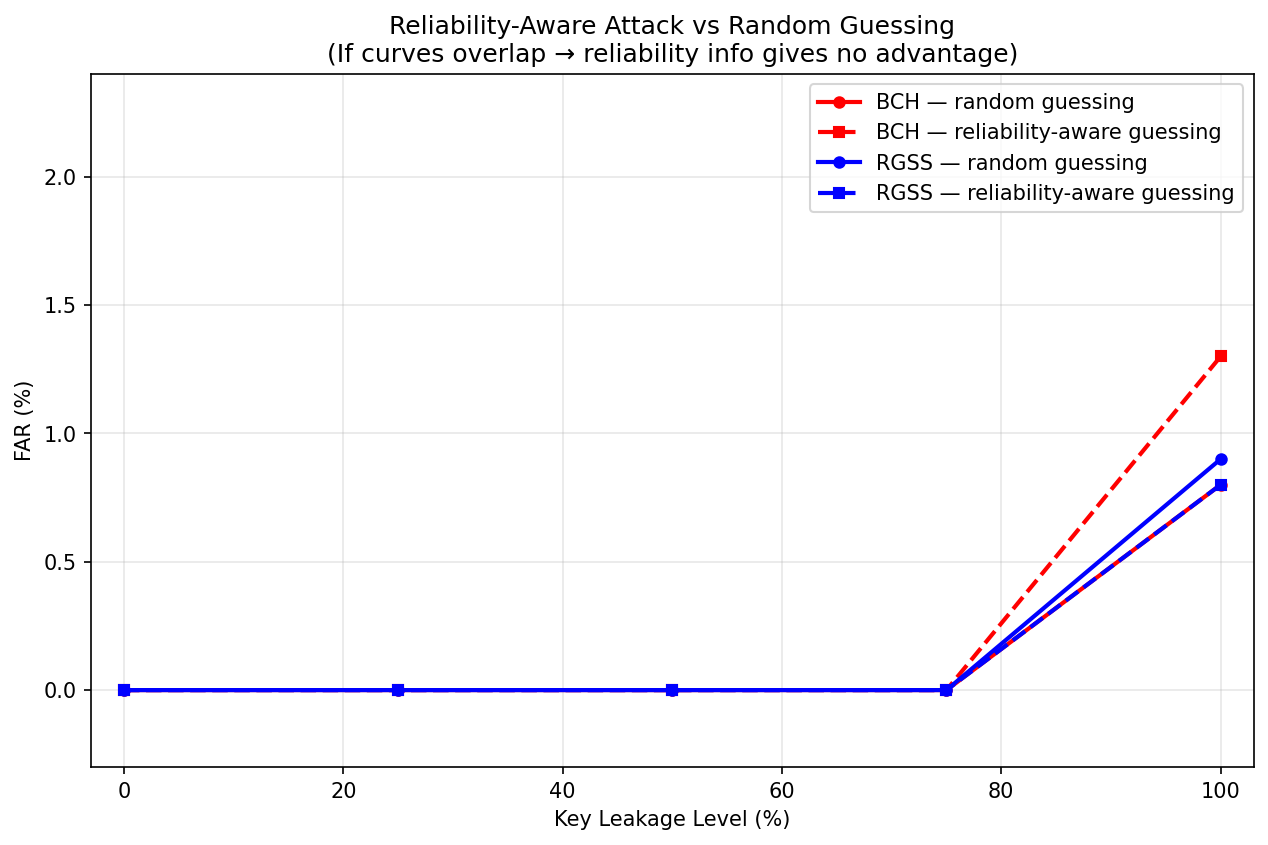
\includegraphics[width=\linewidth]{attack_advanced}
  \caption{FAR comparison for standard partial key leakage and
  reliability-aware guessing attack (BCH and RGSS, G=512).}
  \label{fig:attack_adv}
\end{figure}

\noindent\textbf{Partial key leakage.}
Fig.~\ref{fig:keyleak} shows that both BCH and RGSS yield no successful
attack for 0\%--90\% key leakage (0 successes in 1,000 trials each),
confirming that authentication security is grounded in biometric uniqueness.
At 100\% key leakage (stolen-key), FAR rises to ${\approx}1.1\%$--$1.2\%$,
still low because the adversary must present a fingerprint close to
the enrolled one.

\noindent\textbf{Old-template-assisted attack.}
An adversary holding old template $T_1$ (under key $k_1$) attempts
to authenticate against the new template (under key $k_2$).
No successful attack was observed for BCH in 1,000 independent trials, directly validating the
revocability property: the Hamming distance between $T_1$ and
$T_2$'s helper data is ${\approx}50\%$, beyond BCH correction range.

\noindent\textbf{Reliability-aware guessing attack.}
An adversary aware of RGSS's preference for high-confidence bits
attempts to exploit population-level reliability statistics
when guessing the unknown portion of the key.
Fig.~\ref{fig:attack_adv} shows no successful attack at 0\%--90\% leakage,
identical to standard random guessing, confirming that reliable
bits carry no population-level predictability advantage
(see Section~\ref{sec:exp:entropy}).

\subsection{Helper-Data Leakage, Threat-Model Boundary, and Limitations}
\label{sec:exp:helper}

Under the threat model of Section~\ref{sec:system}, the stored
record $(h, c, \mathcal{R}, \text{SHA256}(s))$ is fully visible to
the adversary.
This section evaluates how much advantage that visibility provides.

\begin{figure}[!t]
  \centering
  \subfloat[FAR under helper-known attack.]%
    {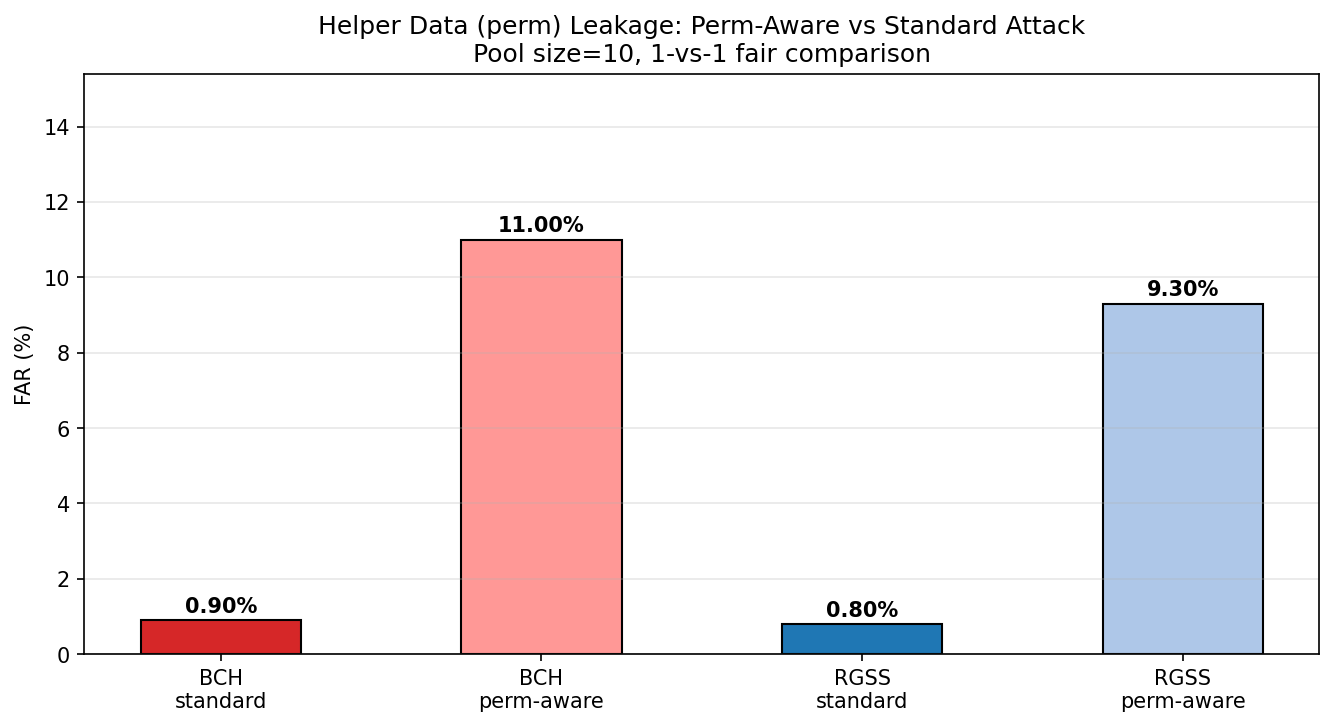
\includegraphics[width=0.48\linewidth]{helper_attack}%
     \label{fig:helper_far}}
  \hfil
  \subfloat[Reliable-position Jaccard similarity.]%
    {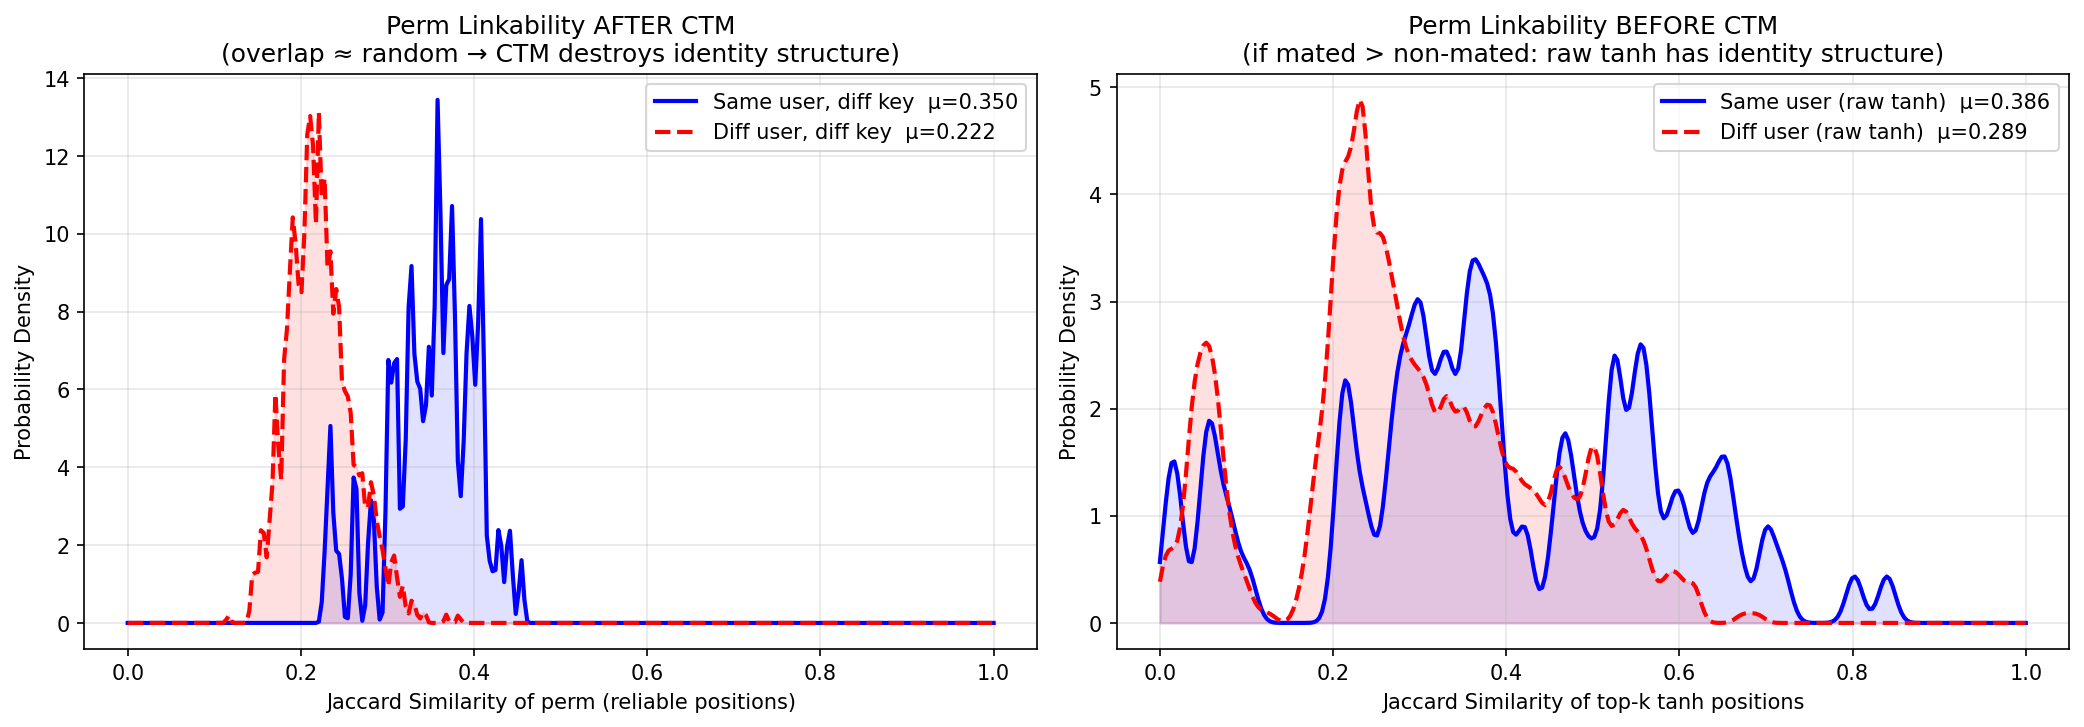
\includegraphics[width=0.48\linewidth]{helper_linkability}%
     \label{fig:helper_link}}
  \caption{Helper data leakage analysis.
  (a)~FAR rises by ${\approx}8$--$10$ percentage points when the
  permutation is exposed (perm-aware attack), but this requires
  leaking the CTM key $\kappa$, not just the secure sketch.
  (b)~After CTM randomization, mated Jaccard similarity is close to
  the random-overlap baseline, while a residual linkability signal
  remains due to the asymmetric non-mated distribution.}
  \label{fig:helper}
\end{figure}

\noindent\textbf{Structural analysis of helper data.}
By construction, $h[\neg\mathcal{R}] = \mathbf{r}_e[\neg\mathcal{R}]$,
meaning the $G - k$ template positions \emph{outside} the reliable
channel are directly revealed in the stored helper data.
This is a consequence of the zero-padding design choice
($s_\text{pad}[i]=0$ for $i \notin \mathcal{R}$) rather than an
inherent property of fuzzy-commitment schemes in general;
alternative constructions (\eg, syndrome-based sketches) can avoid
this direct disclosure.
We acknowledge this as a threat-model boundary of the current design:
the $G-k$ disclosed bits are drawn from a user-specific,
key-dependent selection of the stable pool.
Under our threat model (where the CTM key $\kappa$ is assumed secret
and not derivable from the stored helper data), these bits alone are
insufficient for an adversary to mount a cross-matching attack on the
raw feature vector.
As the perm-aware attack below shows, the CTM key $\kappa$ must be
additionally compromised before these bits provide any authentication
advantage.

\noindent\textbf{Helper-known impostor attack.}
Table~\ref{tab:helper} compares three knowledge levels.
Exposing the CTM key (perm-aware) raises FAR from 0.8\% to
${\approx}9$--$11\%$.
The risk is comparable for BCH and RGSS ($\Delta{=}10.1\%$ vs.\ $8.5\%$),
confirming that the additional exposure is due to CTM key leakage,
not the RGSS design.
In practice, the CTM key is kept secret and not derivable from
the stored helper data.

\begin{table}[!t]
  \renewcommand{\arraystretch}{1.25}
  \caption{Helper-Known Impostor Attack FAR}
  \label{tab:helper}
  \centering
  \begin{tabular}{lcc}
    \toprule
    Attacker Knowledge & BCH FAR & RGSS FAR \\
    \midrule
    Unknown key (standard) & 0.9\% & 0.8\% \\
    Perm-aware (CTM key leaked) & 11.0\% (+10.1\%) & 9.3\% (+8.5\%) \\
    \bottomrule
  \end{tabular}
\end{table}

\noindent\textbf{Reliable-position linkability (Exp.~B).}
Mated Jaccard similarity (same user, different keys) is $0.350 \pm 0.051$,
virtually identical to the random baseline $k/(2G-k) = 0.347$
(Fig.~\ref{fig:helper_link}).
CTM randomization effectively suppresses identity-specific
structure in the reliable-position set.
The residual linkability EER of 9.3\% warrants honest interpretation:
while the asymmetry is \emph{driven} by non-mated pairs having
lower Jaccard than the random baseline ($0.222 < 0.347$), an
adversary who reverses the decision rule can still exploit the
9.3\% distinguishability between mated and non-mated position sets.
We therefore acknowledge that storing $\mathcal{R}$ in the clear
introduces a measurable linkability signal at the reliable-position
level, and recommend masking or hashing $\mathcal{R}$ in security-sensitive
deployments where this residual signal must be eliminated.

\subsubsection{Entropy and Effective Key-Length Interpretation}
\label{sec:exp:entropy}

\begin{figure}[!t]
  \centering
  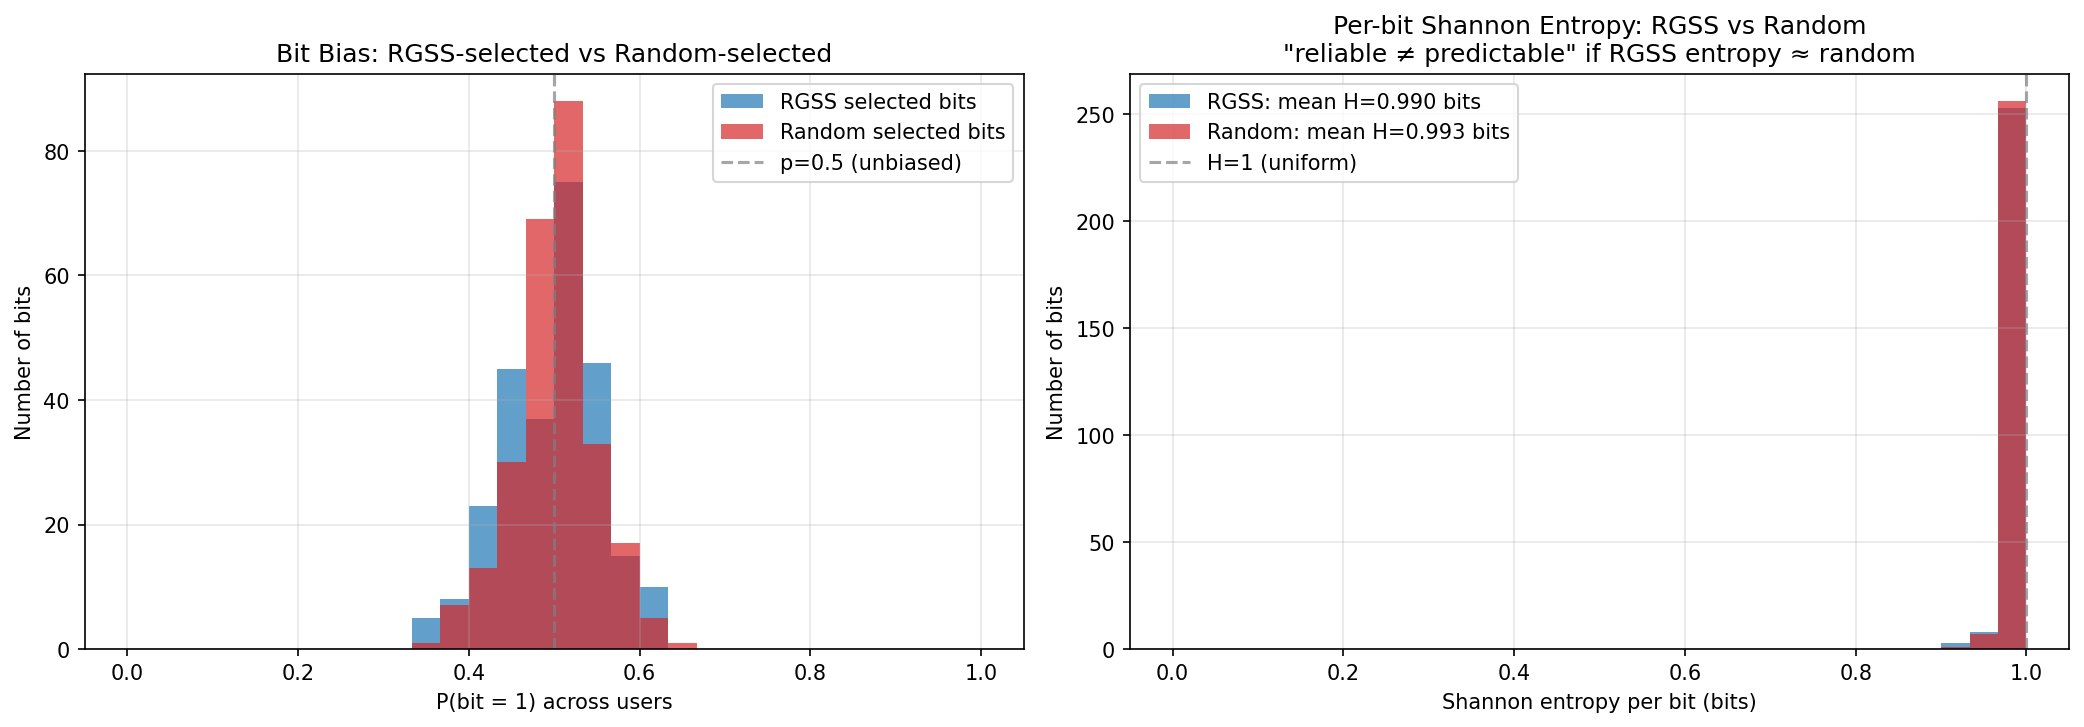
\includegraphics[width=\linewidth]{entropy_comparison}
  \caption{Per-bit Shannon entropy distribution for RGSS-selected
  and randomly-selected bits (G=512, 96 test users, $k=264$).
  The distributions are nearly identical, confirming
  ``reliable $\neq$ predictable.''}
  \label{fig:entropy}
\end{figure}

Fig.~\ref{fig:entropy} and Table~\ref{tab:entropy} report
per-bit entropy statistics for RGSS-selected vs.\ random-selected bits
($k\!=\!264$, 96 test users).
Mean Shannon entropy: $H_\text{RGSS} = 0.9905$\,bits vs.\
$H_\text{random} = 0.9933$\,bits (difference $= -0.003$\,bits).
All selected bits have $H > 0.9$\,bits (100\% in both cases).
The effective entropy upper bound is 261.5\,bits (RGSS) vs.\
262.2\,bits (random), a negligible difference of 0.7\,bits.

This confirms the central claim: selecting reliable bits by tanh
confidence does not bias bit values at the population level.
Reliable bits are stable \emph{for a given user in a given
acquisition} but remain unpredictable across the user population.

\begin{table}[!t]
  \renewcommand{\arraystretch}{1.25}
  \caption{Per-Bit Entropy ($k=264$, 96 Test Users)}
  \label{tab:entropy}
  \centering
  \begin{tabular}{lccc}
    \toprule
    Selection & Mean $H$ & Bits with $H{>}0.9$ & Sum $H$ (bound) \\
    \midrule
    RGSS (proposed) & 0.9905 bits & 100\% & 261.5 bits \\
    Random          & 0.9933 bits & 100\% & 262.2 bits \\
    Difference      & $-0.003$ bits & 0\%  & $-0.7$ bits \\
    \bottomrule
  \end{tabular}
\end{table}

% ---------------------------------------------------------
\subsection{Exp.~9 — Cross-Dataset Generalization}
\label{sec:exp:cross}
% ---------------------------------------------------------

\begin{figure}[!t]
  \centering
  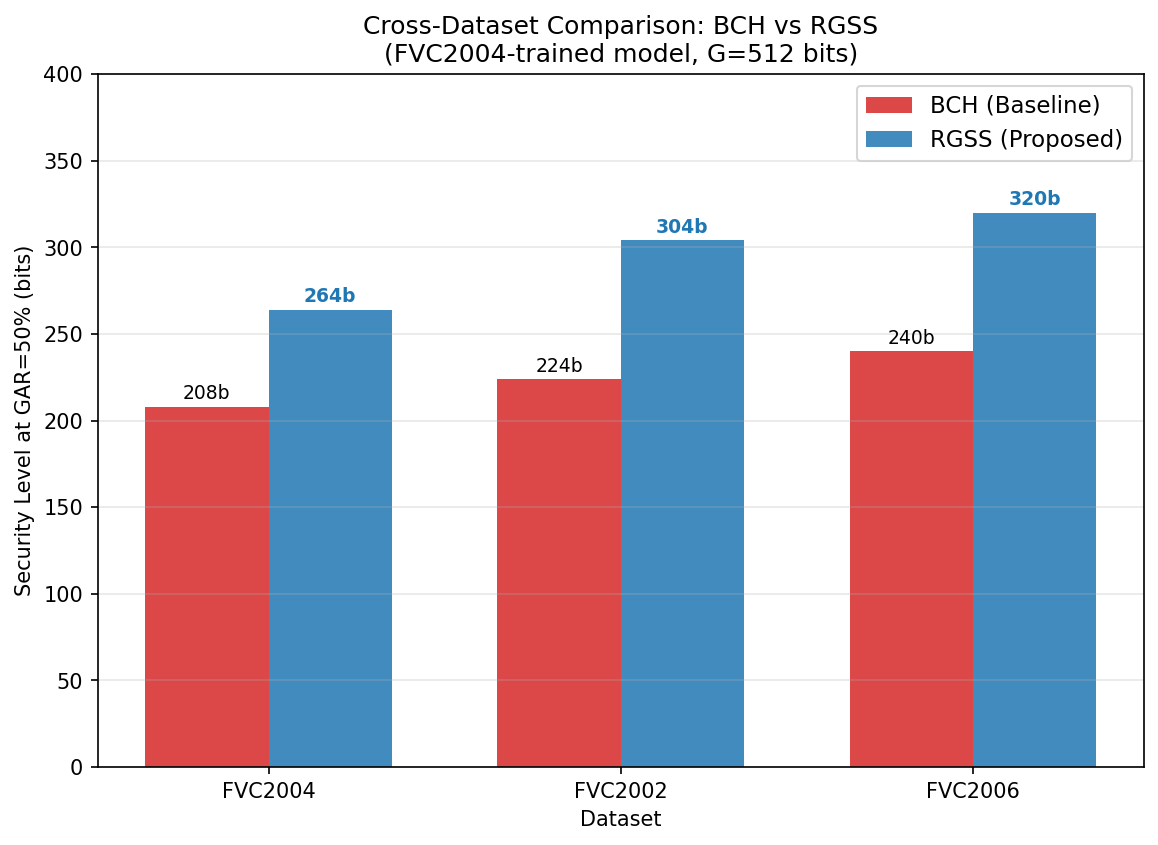
\includegraphics[width=\linewidth]{cross_dataset_summary}
  \caption{$k_{50}$ comparison across three datasets without
  backbone retraining. RGSS consistently outperforms BCH, with
  larger gains on unseen datasets.}
  \label{fig:cross}
\end{figure}

Table~\ref{tab:cross} and Fig.~\ref{fig:cross} evaluate
cross-dataset generalization.
On FVC2002 (unseen, $\bar{p}\!=\!18.06\%$), RGSS achieves
$k_{50}\!=\!304$\,bits vs.\ BCH $k_{50}\!=\!224$\,bits ($+80$\,bits);
at $k\!=\!208$, GAR rises from 63.9\% (BCH) to 85.6\% (RGSS).
On FVC2006 (unseen, $\bar{p}\!=\!16.43\%$), RGSS $k_{50}\!=\!320$
vs.\ BCH $k_{50}\!=\!240$ ($+80$\,bits);
at $k\!=\!208$, GAR rises from 72.9\% (BCH) to 90.2\% (RGSS).
The larger $k_{50}$ advantage on unseen datasets (vs.\ $+56$\,bits on FVC2004)
and the consistently high GAR across all three datasets confirm that RGSS's
reliable-channel concentration generalizes well to new sensors and acquisition
conditions, with lower genuine flip rates amplifying the benefit.
Authentication accuracy and the GAR--key-length tradeoff are thus
simultaneously stable across datasets without any backbone retraining.

\begin{table}[!t]
  \renewcommand{\arraystretch}{1.25}
  \caption{Cross-Dataset Generalization (G=512, no backbone retraining).
  $k_{50}$: last $k$ with GAR$\ge$50\%.
  GAR@208: genuine acceptance rate at $k\!=\!208$ (BCH's FVC2004 operating point).
  FVC2004 GAR@208 values are from an independent evaluation run of Exp.~9;
  minor numerical differences from Table~\ref{tab:sstm} ($\le\!1.2\%$)
  reflect random variation in CTM key sampling between runs.}
  \label{tab:cross}
  \centering
  \begin{tabular}{lccccccc}
    \toprule
    Dataset & $\bar{p}$ & \multicolumn{2}{c}{$k_{50}$ (bits)} & $k_{50}$ Gain
            & \multicolumn{2}{c}{GAR@208\,(\%)} \\
    \cmidrule(lr){3-4}\cmidrule(lr){6-7}
    & & BCH & RGSS & & BCH & RGSS \\
    \midrule
    FVC2004 (in-dist.) & 19.45\% & 208 & 264 & $+56$ & 53.9 & 86.8 \\
    FVC2002 (unseen)   & 18.06\% & 224 & 304 & $+80$ & 63.9 & 85.6 \\
    FVC2006 (unseen)   & 16.43\% & 240 & 320 & $+80$ & 72.9 & 90.2 \\
    \bottomrule
  \end{tabular}
\end{table}

% ---------------------------------------------------------
\subsection{Exp.~10 — Statistical Significance}
\label{sec:exp:stats}
% ---------------------------------------------------------

\begin{figure}[!t]
  \centering
  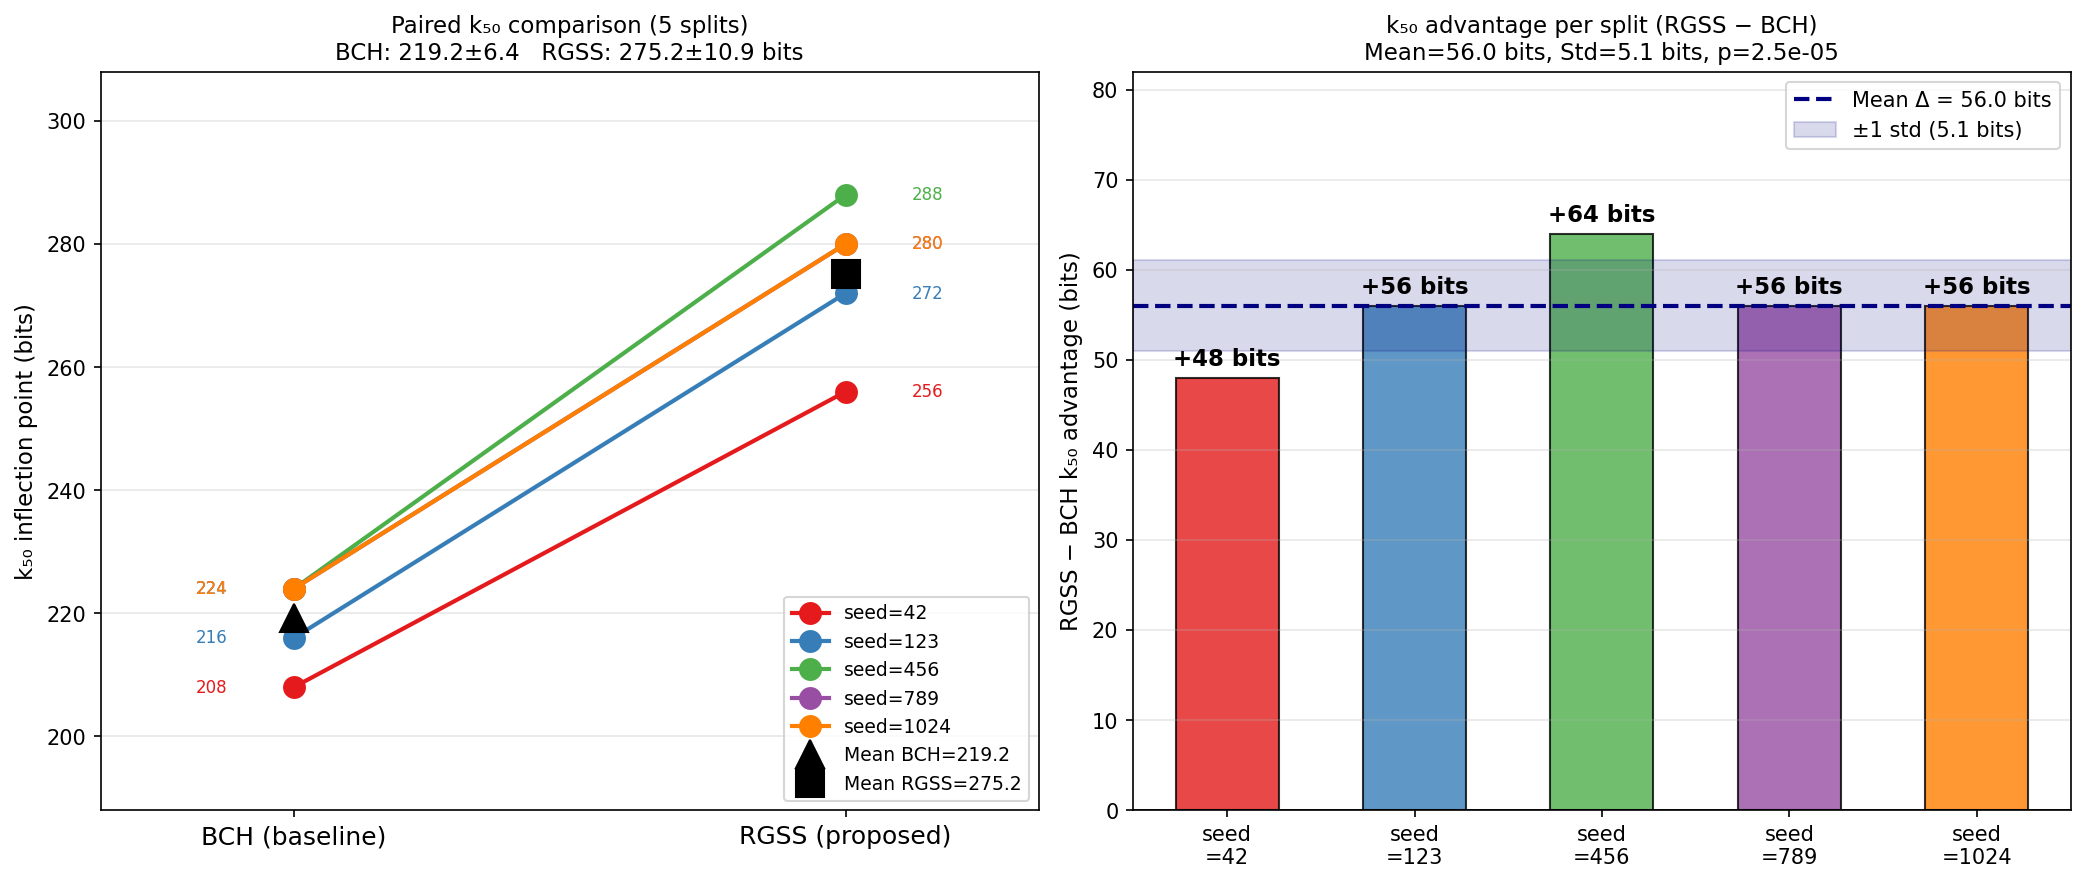
\includegraphics[width=0.9\linewidth]{significance_boxplot}
  \caption{$k_{50}$ values across 5 random train/test splits
  (slope chart: each seed is one colored line;
  bar chart: per-seed RGSS gain over BCH).}
  \label{fig:stats}
\end{figure}

To assess statistical robustness, we fix the VGG-19 backbone and
repeat the GAR--key-length evaluation under 5 independent subject-disjoint splits
(seeds 42, 123, 456, 789, 1024).

BCH $k_{50}$: $219.2 \pm 6.4$\,bits;
RGSS $k_{50}$: $275.2 \pm 10.9$\,bits;
advantage $\Delta$: $56.0 \pm 5.1$\,bits.
Paired $t$-test: $t\!=\!22.14$, $p\!=\!2.5 \times 10^{-5}$.

The gain is consistent across all splits (+48 to +64\,bits) and
highly significant.
This result supports the following notation used hereafter:
\emph{RGSS achieves $k_{50} = 275.2 \pm 10.9$\,bits, consistently
outperforming BCH by $56.0 \pm 5.1$\,bits over five random seeds
(paired $t$-test, $p < 0.001$).}

% =========================================================
%  VI. CONCLUSION
% =========================================================
\section{Conclusion}
\label{sec:conclusion}

We have presented RGSS, a reliability-guided secure sketch for
deep fingerprint template protection.
By leveraging sample-wise tanh confidence from a deep hashing network
to select reliable BCH channel positions at enrollment time, RGSS
consistently advances the GAR--key-length tradeoff by 56--80\,bits
over BCH baselines across three fingerprint datasets, surpassing
both population-level flip-rate guidance and the test-set population flip-rate baseline.
Security evaluations support revocability, indicate low
template-level linkability under the evaluated distance-based
protocol ($D_\text{sys}\!=\!0.046$), and show no successful attacks
under the evaluated advanced-attack settings, while per-bit entropy
remains comparable to random selection.
\noindent\textbf{Limitation.}
The current zero-padding helper-data construction exposes $G-k$
template bits outside the reliable channel and stores
$\mathcal{R}$ in the clear, which creates a measurable
reliable-position linkability signal.
Future work should replace this helper-data design with
syndrome-based sketches and protected representations of
$\mathcal{R}$ to reduce this leakage boundary.
These results collectively establish RGSS as an effective
sample-adaptive secure sketch for deep binary biometric templates.

Future work includes extending RGSS to other deep biometric
modalities (iris, face), integrating convolutional reliability
maps for spatial feature localization, and investigating stronger
ECC codes (e.g., LDPC) once template lengths are sufficiently large.

% =========================================================
%  APPENDIX (optional)
% =========================================================
% \appendices
% \section{Proof of Expected Error Reduction}
% \TODO{formal proof of Eq.~\eqref{eq:expected_errors}}

% =========================================================
%  ACKNOWLEDGMENT
% =========================================================
\section*{Acknowledgment}
The authors would like to thank the members of the Multimedia
Communication and Pattern Recognition Laboratory at BUPT for helpful
discussions.

% =========================================================
%  REFERENCES
% =========================================================
\bibliographystyle{IEEEtran}
\bibliography{IEEEabrv,references}

% =========================================================
%  AUTHOR BIOGRAPHIES
% =========================================================
\begin{IEEEbiographynophoto}{Yubo Gao}
received the B.Eng.\ degree from Beijing University of Posts and
Telecommunications (BUPT), Beijing, China, where he is currently
pursuing the M.S.\ degree with the School of Artificial Intelligence.
His research interests include biometric template protection,
deep hashing, and cancelable biometrics.
\end{IEEEbiographynophoto}

\begin{IEEEbiographynophoto}{Zhe Cui}
(Member, IEEE) received the B.S.\ degree from the Department of
Physics, Tsinghua University, in 2014, and the M.Eng.\ and Ph.D.\
degrees from the Department of Automation, Tsinghua University,
in 2017 and 2021, respectively.
He is currently an Associate Professor with the School of Artificial
Intelligence, Beijing University of Posts and Telecommunications,
Beijing, China.
His research interests include fingerprint recognition, computer
vision, and pattern recognition.
(Corresponding author: Zhe Cui.)
\end{IEEEbiographynophoto}

\begin{IEEEbiographynophoto}{Fei Su}
(Member, IEEE) received the Ph.D.\ degree in communication and
electrical systems from the Beijing University of Posts and
Telecommunications (BUPT), China, in 2000.
She was a Visiting Scholar with the Department of Electrical and
Computer Engineering, Carnegie Mellon University, USA, from 2008 to
2009.
She is currently a Professor with the Multimedia Communication and
Pattern Recognition Laboratory, BUPT.
She has authored and coauthored more than 150 journal articles and
conference papers and some textbooks.
Her current interests include pattern recognition, image and video
processing, and biometrics.
\end{IEEEbiographynophoto}

\end{document}
